\documentclass[12pt, a4paper]{article}
\usepackage{listings}
\usepackage{sourcecodepro}
\usepackage{xcolor}
\definecolor{backcolour}{rgb}{0.95,0.95,0.92}
\definecolor{codegray}{rgb}{0.5,0.5,0.5}
\lstdefinestyle{mystyle}{
    backgroundcolor=\color{backcolour},   
    numberstyle=\tiny\color{codegray},
    keywordstyle=\color{black}\bfseries,
    breakatwhitespace=false,         
    breaklines=true,                 
    captionpos=b,                    
    keepspaces=true,                 
    numbers=left,                    
    numbersep=5pt,                  
    showspaces=false,                
    showstringspaces=false,
    showtabs=false,                  
    tabsize=2,
	basicstyle=\small\ttfamily
}
\lstset{style=mystyle}
\usepackage[dutch]{babel}
\usepackage{array}
\usepackage{adjustbox}
\usepackage{wrapfig}
\usepackage{stix}
\usepackage{amsmath}
\newcommand*{\ora}{\overrightarrow}
\usepackage{tikz}
\usepackage{pgfplots}
\usepackage{algorithm}
\usepackage[noend]{algpseudocode}
\usepackage{graphicx}
\graphicspath{{images/}}
\usepackage{chngcntr}
\usetikzlibrary{calc}
\usetikzlibrary{angles}
\counterwithin{figure}{section}
\title{Efficiëntie van raymarching in renderen}
\author{Taeke Roukema}
\date{December 2023}

\makeatletter
\def\BState{\State\hskip-\ALG@thistlm}
\makeatother

\begin{document}
\maketitle
\begin{abstract}
Renderen met raymarching
\end{abstract}
\clearpage
\tableofcontents{}
\clearpage
\section{Voorwoord}
\clearpage
\section{Inleiding}
\subsection{Introductie onderwerp}

Renderen is overal. Als je je telefoon opent zie je allerlei gerenderde vormen. Bij het ontbijt zijn verpakkingen volgeprint met teksten die met de computer getekend zijn. Als je langs een bouwterrein loopt zie je hyperrealistische visualisaties van de architectuur. Moderne blockbuster-films zitten tegenwoordig bomvol CGI\footnote{\textbf{C}omputer \textbf{G}enerated \textbf{I}magery}. En er zijn al tientallen jaren films te zien die helemaal door de computer gemaakt zijn. 

\begin{wrapfigure}{s}{0.5\textwidth}
    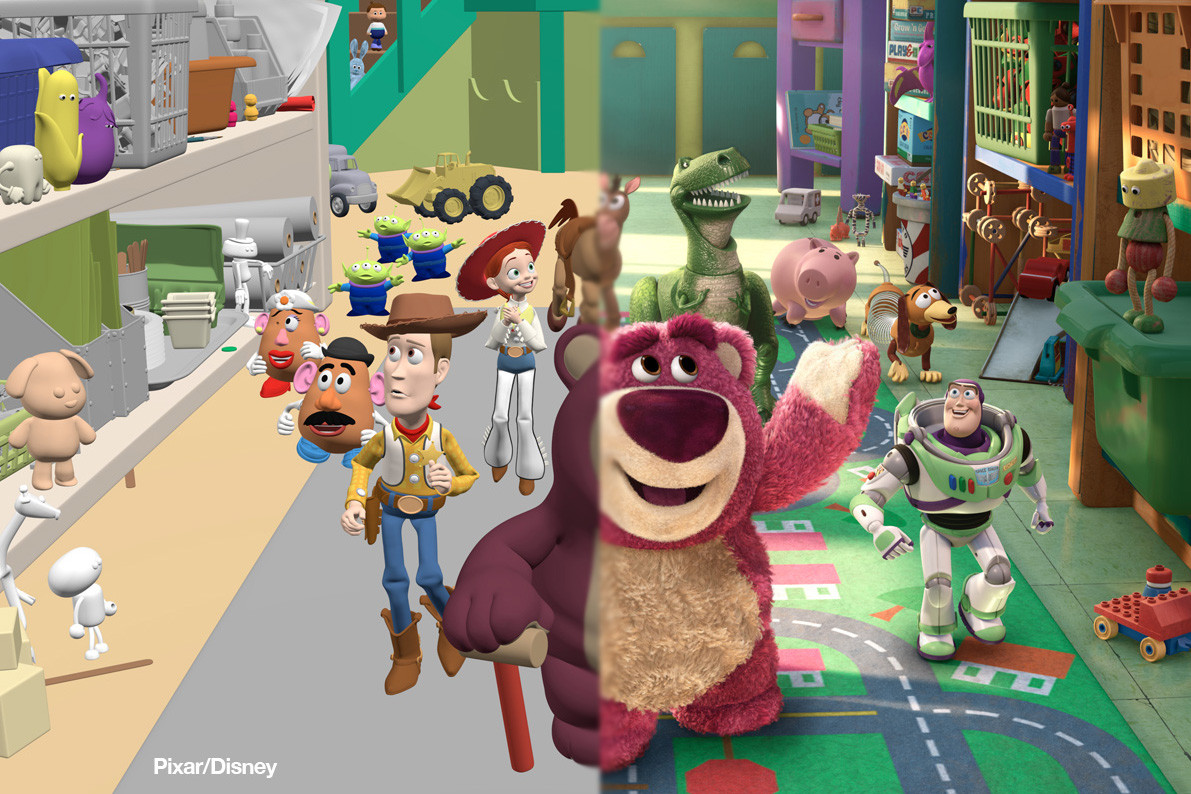
\includegraphics[width=1\linewidth]{toystory3comparison.jpg}
    \caption{Een frame uit Toy Story 3, aan de linkerkant worden geen lichtberekeningen gedaan, en aan de rechterkant wel.}
    \label{fig:toystory3}
\end{wrapfigure}

Voor Toy Story 3 (Figuur \ref{fig:toystory3}) werd er gemiddeld zeven uur over gedaan om een frame te renderen \cite{HowToyStory3WasMade}. En dat terwijl er gebruik werd gemaakt van twee gigantische render farms\footnote{Een computercluster speciaal gemaakt voor het renderen van CGI, de term was geïntroduceerd in de productie voor Bored Room\cite{MakingOfBoredRoom}}. Het renderen van films kost niet alleen enorm veel tijd, maar ook veel energie. Het is dus belangrijk dat het zo efficiënt mogelijk gebeurd. Er wordt over de hele wereld voortdurend onderzoek gedaan naar manieren om dit proces efficiënter te maken en te verbeteren. De opkomst van kunstmatige intelligentie begint al bewegingen te maken in de wereld van CGI \cite{NeRFactor}. Maar er wordt ook voortdurend voortuitgang gemaakt op fundamentelere manieren. Zo zijn er de afgelopen vijf jaar GPU's\footnote{\textbf{G}raphics \textbf{P}rocessing \textbf{U}nit} van Nvidia op de markt gekomen met ingebouwde support voor realtime raytracing\cite{NvidiaRTX}. Door op het hardware niveau de chips zo te ontwerpen dat ze heel goed zijn in bepaalde berekeningen die gebruikt worden voor het simuleren van licht kunnen GPU's gebruikt worden om voormalig minutendurende processen meer dan zestig keer per seconde uit te voeren. 
\begin{figure}[h]
    \centering
    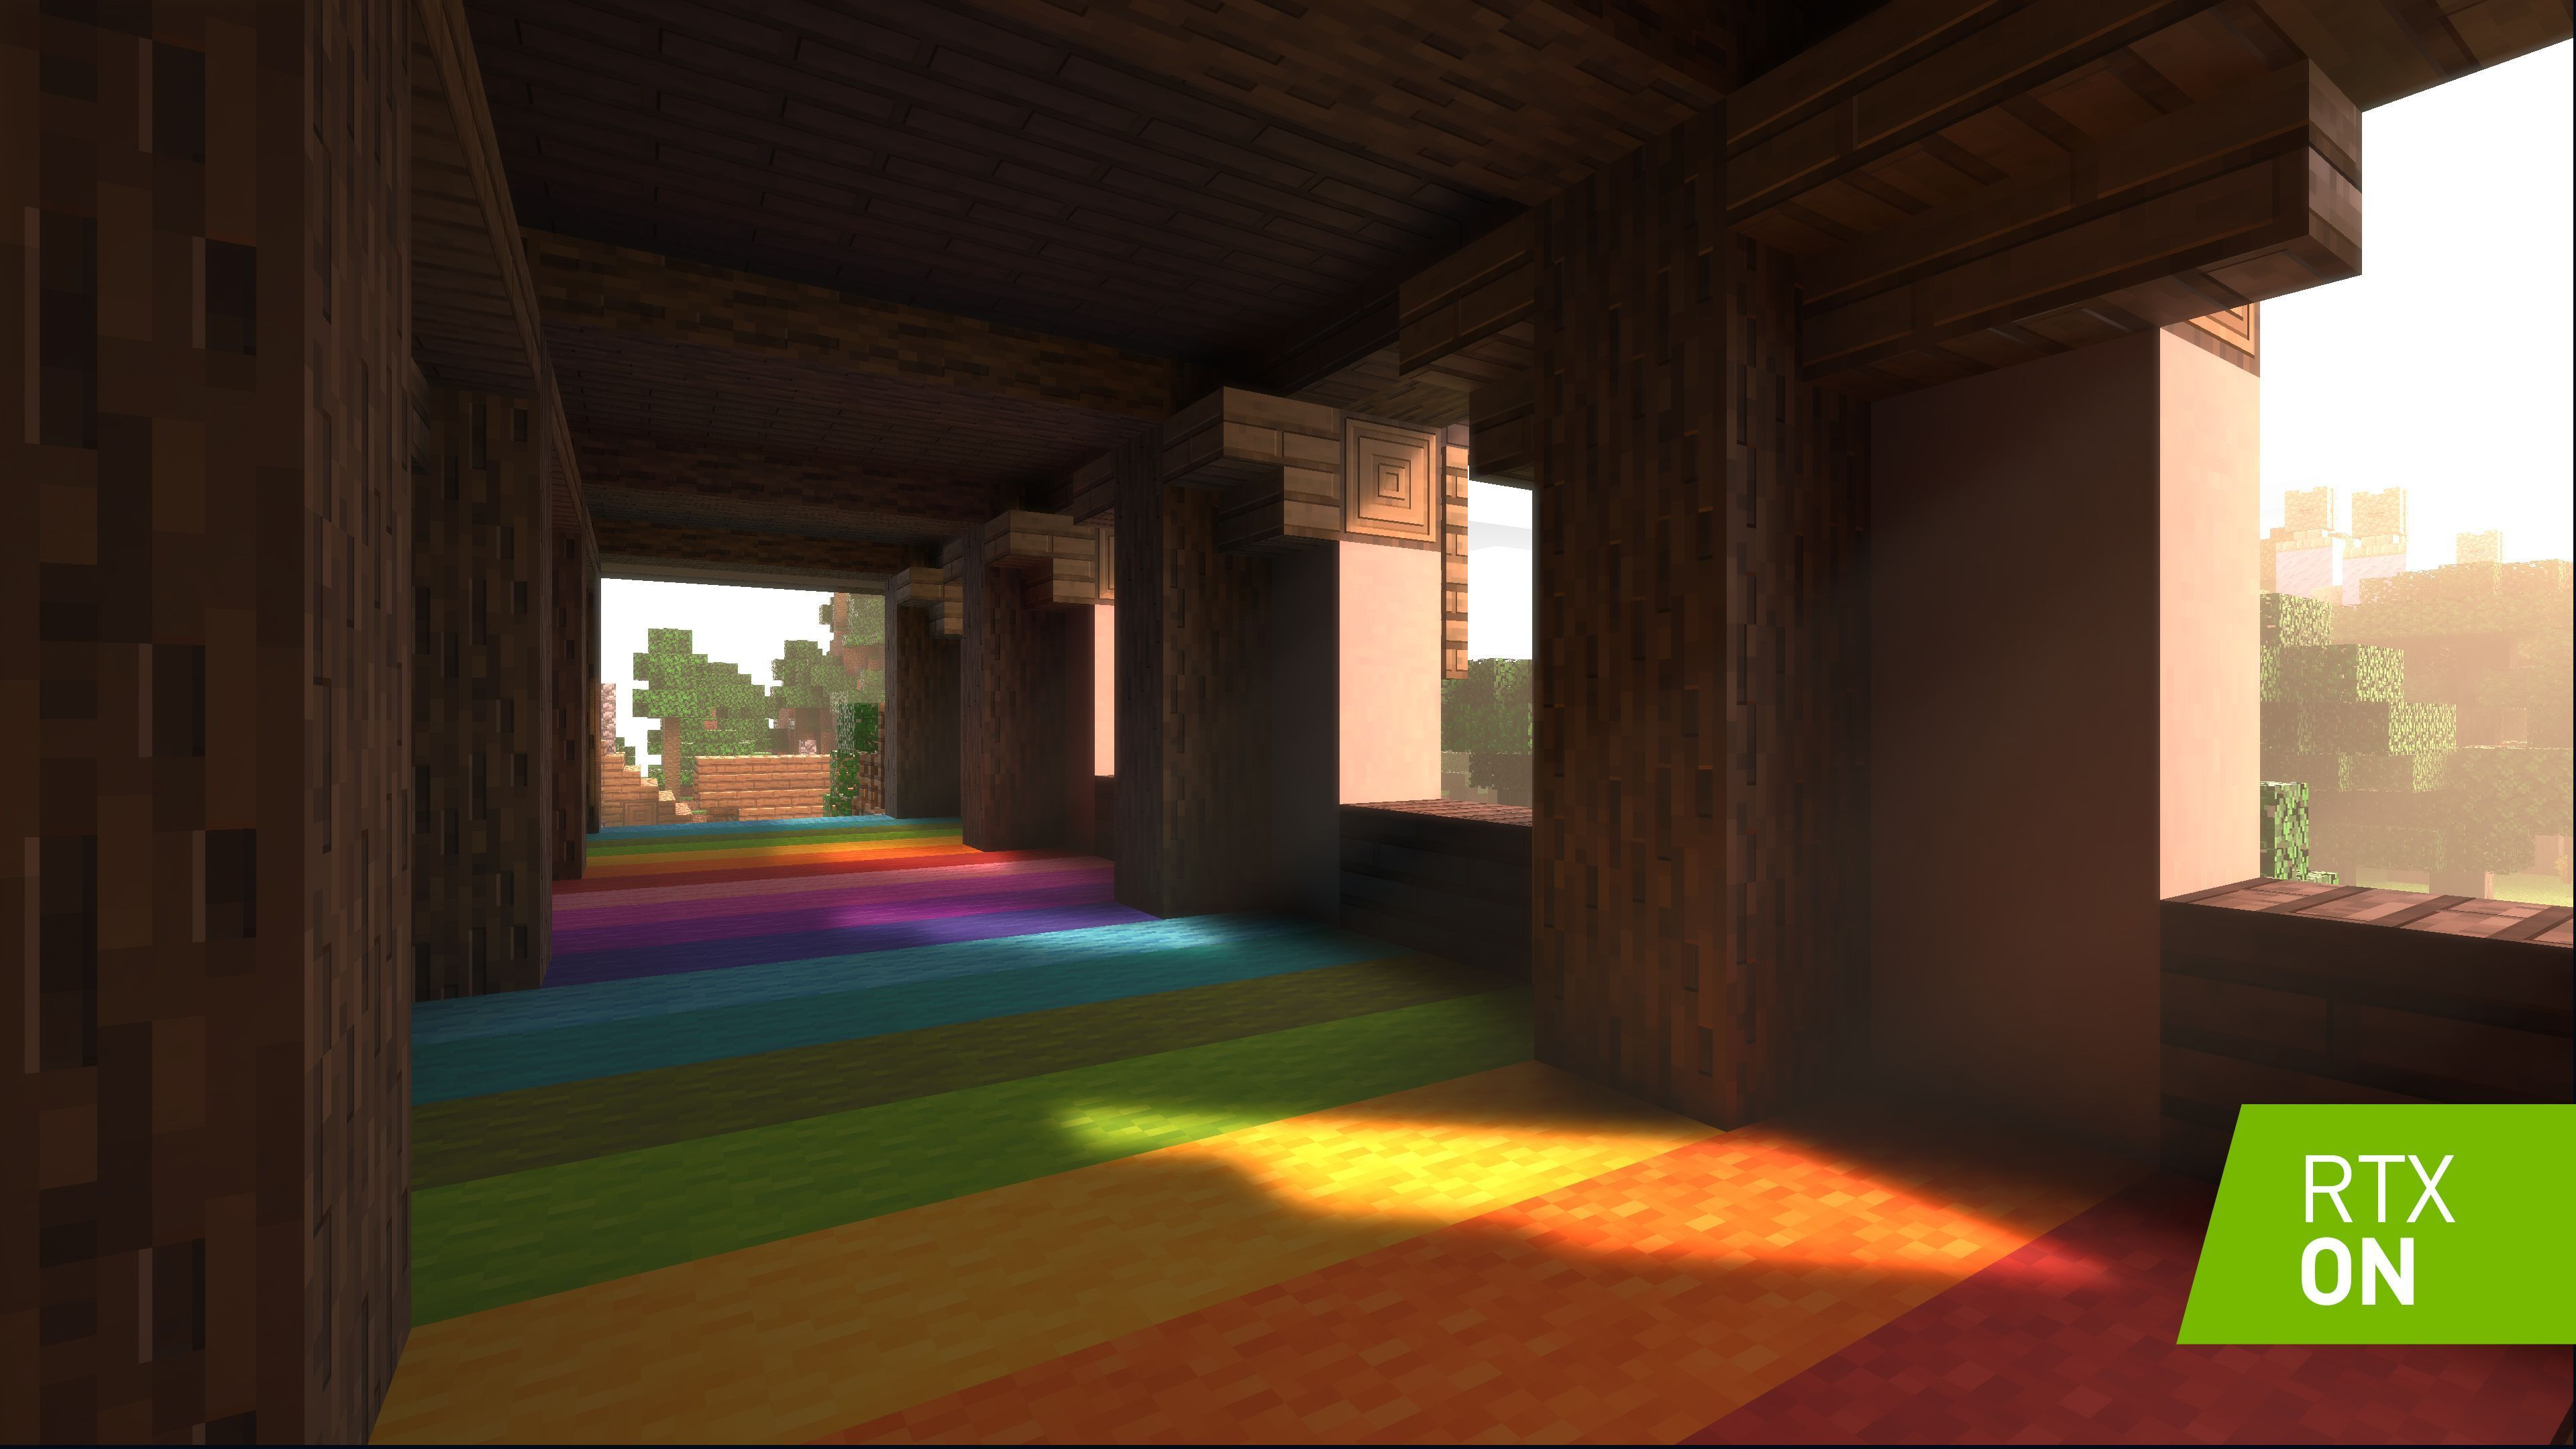
\includegraphics[width=0.5\textwidth]{minecraftrtx.jpg}
    \caption{De videogame Minecraft kan gebruik maken van Nvidia GPU's om realtime lichtsimulaties te berekenen.}
    \label{fig:minecraftrtx}
\end{figure}

Er zijn twee belangrijke maatstaffen waarmee we de efficiëntie van een renderalgoritme kunnen meten. De eerste is vanzelfsprekend: snelheid. Als een frame sneller gerenderd is wordt er minder energie gebruikt en zijn we goedkoper uit. Maar ook geheugenbezetting is belangrijk om rekening mee te houden. Het geheugen is simpelweg de plaats in de computer waar alle informatie wordt opgeslagen. Als je berekeningen doet moet je ergens de resultaten tussendoor opslaan. Complexe scènes kunnen enorm veel details hebben, die allemaal in het geheugen opgeslagen zijn. Het is niet gratis om extra geheugen toe te voegen, het is dus belangrijk om de geheugenbezetting te minimaliseren. 

Vrijwel alles is tegenwoordig op een manier gerenderd. Objecten zijn gedesigned met gebruik van CAD\footnote{\textbf{C}omputer \textbf{A}ided \textbf{D}esign}. Besturingssytemen runnen op een grafische shell. En een meerendeel van advertenties gebruikt CGI.
% Beschrijven hoe renderen voorkomt in het dagelijkse leven

Volgens Peter Collinridge\cite{ScienceBehindPixarRendering} gebruikt de render farm van pixar 24000 processor cores verdeeld over 2000 computers. Er wordt dus waarschijnlijk gebruik gemaakt van computers met \(24000/2000=12\) cores. De Ryzen 9 5900x is een voorbeeld van een processor met 12 cores, het energiegebruik zal niet exact hetzelfde zijn maar het ligt bij elkaar in de buurt. De 5900x gebruikt 105 Watt. \(105W\cdot 2000\approx 2,10\cdot 10^5W\). Volgens dezelfde bron kostte het renderen van Monster's University twee jaar. Dat is \(2\cdot 365\cdot 24\approx17520h\). \[210kW \cdot 17520h\approx 3679200kWh\] Een gemiddeld huishouden in Nederland gebruikt 2479 kWh per jaar. Dit betekent dat het renderen van Monster's University \(3679200/2479\approx 1484\) huishoudens een jaar lang van energie had kunnen voorzien. En dat is alleen nog maar de processorkracht, er gaat ook nog energie naar de moederborden, het geheugen, de koeling en de harde schijven. Kortom, er valt een hoop te besparen.
% Beschrijven hoeveel energie renderen kan kosten
% Impact klimaat
\subsection{Onderzoeksvraag/deelvragen}
\subsubsection{Hoofdvraag WIP}
In welke situaties is raymarching een efficiëntere rendertechniek dan polygonaal renderen?

Vergelijking van twee rendermethoden in rendersnelheid en geheugenbezetting.

Vergelijking van raymarching en polygonaal renderen in rendersnelheid en geheugenbezetting.

Hoe wegen raymarching en polygonaal renderen tegen elkaar op in rendersnelheid en geheugenbezetting?
\subsubsection{Deelvragen WIP}
\begin{itemize}
\item{Hoe beschrijf je een driedimensionale vorm?}
\item{Hoe werkt raytracing?}
\item{Hoe werkt raymarching?}
\item{Hoe werkt rasterization?}
\item{Hoe beschrijf je een vorm zodat het gerenderd kan worden met raymarching?}
\item{Hoeveel geheugen neemt polygonaal renderen in?}
\item{Hoeveel geheugen neemt renderen met raymarching in?}
\item{Hoe snel is renderen met raymarching vergeleken met polygonaal renderen?}
\item{Hoe kan je met raymarching objecten modelleren?}
\end{itemize}
\clearpage
\section{Theorie}
\subsection{Wat is renderen?}
Renderen is, in feite, het weergeven van een representatie van een concept op een beeldscherm. Wij zijn voortdurend bezig met het interacteren met computers, en die interactie verloopt via het beeldscherm. Maar de computer kan uit zichzelf niet zomaar alles tekenen. Daar worden allemaal algoritmes voor geschreven. Een voorbeeld van zo'n algoritme is het tekenen van een rechthoek. In pseudocode zou je dat als volgt voor kunnen stellen:
\begin{algorithm}
\caption{Rechthoek Algoritme}\label{euclid}
\begin{algorithmic}[1]
\Procedure{DrawRectangle}{x1, x2, y1, y2}
    \For{$x \gets x1$ to $x2$}             
	    \For{$y \gets y1$ to $y2$}             
		\State $\text{draw pixel at }(x, y)$
	    \EndFor
    \EndFor
\EndProcedure
\end{algorithmic}
\end{algorithm}

Het algoritme beschouwt elke pixel die binnen de rechthoek valt en kleurt die pixel. In dit geval wordt dat gedaan door twee loops, die samen alle mogelijke combinaties van x- en y-coördinaten doorlopen. 

Renderen omvat, in principe, niks anders dan het aansturen van individuele pixels. Zo'n pixel heeft op de meeste moderne beeldschermen drie waarden die de kleur aansturen: R, G en B, die respectievelijk staan voor rood, groen en blauw. Ze kunnen een geheel getal tussen de 0 en 255 aannemen wat resulteert in \(2^{24}\) mogelijke kleuren.
\begin{figure}[h]
\centering
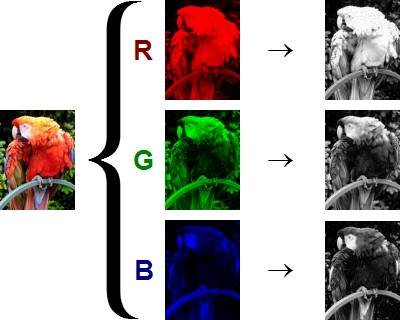
\includegraphics[width=0.5\textwidth]{RGB_channels_separation.png}
\caption{De kleuren in een foto kunnen opgesplitst worden in rode, groene en blauwe kanalen.}
\label{fig:rgb_separated}
\end{figure}

Renderen doen we op een twee-dimensionaal beeldscherm. Dat betekent dat de positie van elke pixel te beschrijven is met twee waarden. Maar de wereld om ons heen kent niet twee, maar drie ruimtelijke dimensies. Door licht dat op ons netvlies valt na weerkaatst te zijn door verschillende objecten kunnen wij die wereld representeren in onze hersenen op een tweedimensionale manier. Camera's gebruiken een gelijksoortige techniek, de lens neemt het licht en projecteert het op een sensor die de intensiteit en de kleur waarneemt. Met het renderen van driedimensionale objecten proberen we deze processen na te bootsen. 

\subsection{De rendervergelijking}
\[
L_{\text{o}}(\mathbf x, \omega_{\text{o}}, \lambda, t) = L_{\text{e}}(\mathbf x, \omega_{\text{o}}, \lambda, t) \ + \int_\Omega f_{\text{r}}(\mathbf x, \omega_{\text{i}}, \omega_{\text{o}}, \lambda, t) L_{\text{i}}(\mathbf x, \omega_{\text{i}}, \lambda, t) (\omega_{\text{i}}\cdot\mathbf n) \operatorname d \omega_{\text{i}}
\]

\subsection{Wat is rasterization?}
In de vroege jaren van de ontwikkeling van de computer was de rekenkracht miniscuul vergeleken met waar we vandaag de dag toegang tot hebben. Gordon Moore, mede-oprichter van Intel en legendarische informaticus, stelde in 1965 Moore's Law voor (al had het toen nog een andere naam). Moore's Law stelt dat elke twee jaar het aantal transistors in een \emph{integrated circuit} verdubbelt \cite{CrammingComponents}. Dit betekent dus dat 40 jaar geleden de computers \(\frac{1}{2^{20}}\) keer zoveel rekenkracht hadden. Wat ongeveer één miljoenste is. Het was toen simpelweg niet mogelijk om algoritmes zoals raytracing toe te passen, omdat de complexiteit van dat soort algoritmes de capaciteit van de computers ver te boven gingen.

De oplossing was relatief simpel, in plaats van voor elke pixel te checken of er een object in de weg zit kijk je alleen maar naar de positie van de hoeken van een vorm. Als je daar vervolgens de schermcoördinaten van hebt kan je de vorm gewoon invullen, wat een vrij goedkoop proces is.

Rasterization is de standaard in de wereld van realtime renderen, vanwege het significante voordeel op de snelheid. Echter kent de methode veel nadelen. De belangrijkste van deze nadelen is het feit dat het beeld altijd een benadering zal zijn van de echte wereld. Het licht wordt niet gesimuleerd, er worden verschillende trucs gebruikt om te doen alsof het echt is maar het zal nooit echt kunnen zijn. 
\subsection{Wat is raytracing?}

Om licht realistischer te simuleren ligt het voor de hand om vanuit elke lichtbron miljoenen lichtstralen af te vuren, die laat je door de scène kaatsen totdat ze het zichtveld van de observeerder raken. In theorie is dit de realistische benadering, en ook exact wat de rendervergelijking op het eerste oog impliceert. Deze methode wordt \emph{photon tracing} genoemd, naar de naam van lichtdeeltjes: fotonen. Maar in de werkelijkheid is dit vrijwel onmogelijk. Maar een klein gedeelte van de lichtstralen bereikt daadwerkelijk ooit de camera, wat betekent dat verreweg de meeste berekeningen die gemaakt worden geen invloed hebben op het uiteindelijke eindbeeld. 

Om dit probleem op te lossen vuren we de stralen niet af vanuit de lichtbronnen, maar vanuit de camera. Voor elke pixel op het scherm wordt een straal door het zichtveld afgevuurd. Als die straal een object raakt kaatsen we die vervolgens af naar de lichtbronnen om te kijken hoe sterk die pixel belicht moet zijn, en of er eventueel een object in de weg zit die een schaduw zou werpen. Bovendien kunnen we de stralen door laten kaatsen tussen objecten, hiermee kunnen we een model van reflectie benaderen. 

\begin{figure}[h]
    \centering
    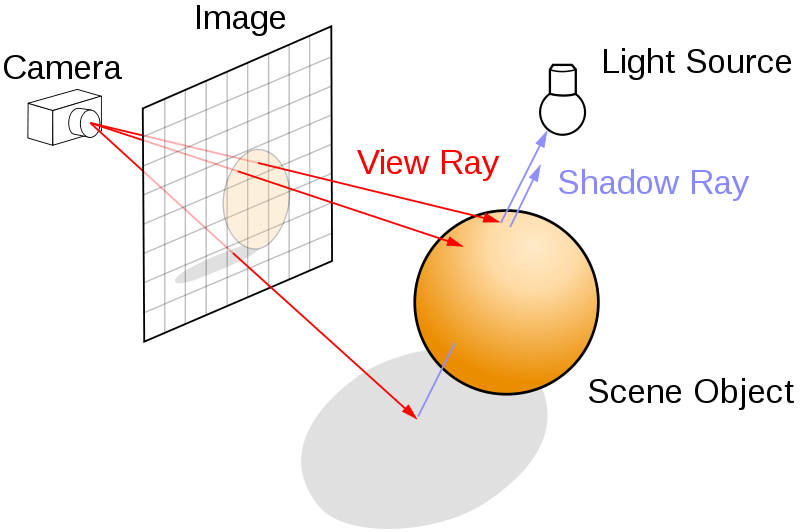
\includegraphics[width=0.75\textwidth]{raytracing_diagram.png}
    \caption{Een diagram die laat zien hoe raytracen werkt}
    \label{fig:raytracing_diagram}
\end{figure}

Het renderen wordt met deze methode al een stuk meer te overzien. Voor het genereren van een plaatje van \(1000\times 1000\) pixels vuren we een miljoen stralen af, wat klinkt alsof het veel is. Maar voor moderne computers is dat zeker haalbaar. Pas als we reflecties toe gaan passen lopen we tegen een klein probleem aan, omdat de rendertijd dan polynomiaal groeit met het aantal objecten in de scène. Dit is omdat we elk object moeten testen met ieder ander, wat zorgt voor een kwadratisch verband.

\subsection{Hoe werkt shading?}
Eén manier om lichtsimulaties te benaderen is het \emph{Phong Reflection Model} \cite{PhongReflectionModel}. Hierbij wordt de belichting van een object opgesplitst in drie delen: Ambient, Diffuse en Specular.
\begin{figure}[h]
\centering
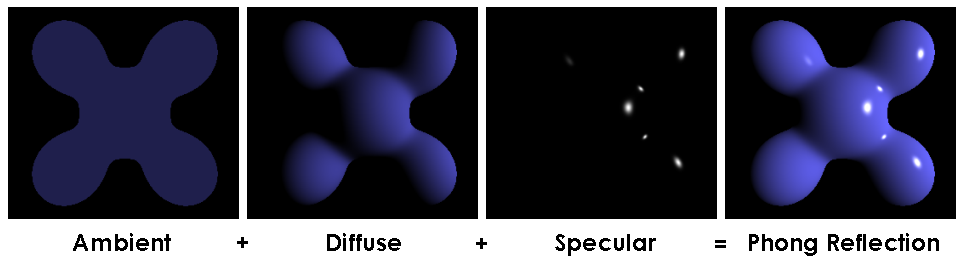
\includegraphics[width=0.8\textwidth]{Phong_components.png}
\caption{De verschillende componenten van het \emph{Phong Reflection Model}.}
\label{fig:phong_components}
\end{figure}

Ambient reflectie staat voor de kleine hoeveelheden licht die eigenlijk altijd wel aanwezig zijn door licht wat door de ruimte heen kaatst. Aangezien het berekenen van deze weerkaatsingen enorm veel rekenkracht kost wordt er uitgegaan van een universele gelijke belichting. 

Diffuse reflectie wordt berekend aan de hand van de hoek tussen het licht op het object en de normaal. Als deze hoek groter is wordt de intensiteit kleiner, omdat het licht meer verdeeld wordt over het oppervlakte. Bij diffuse reflectie ga je ervan uit dat het licht evenveel in elke richting wordt afgekaatst, daarom wordt dit vooral veel voor ruwe oppervlakten gebruikt, waar kleine imperfecties in de textuur ervoor zorgen dat het licht alle kanten op gekaatst wordt.

Bij gladdere oppervlakten is er sprake van specular reflectie. Hier wordt het licht meer gereflecteerd in de tegenovergestelde richting dat het binnenkomt tegenover de normaal. 

Als deze drie technieken samengevoegd worden krijg je een vrij accurate benadering van de beweging van echt licht.

\subsection{Wat is global illumination?}
De methode die hierboven beschreven staat is niet perfect. Als een straal een object ziet tussen het raakpunt en de lichtbron wordt dat punt helemaal niet belicht. Dit is omdat het algoritme niet berekent hoe het licht door de kamer heen kaatst vanuit de lichtbron. Dat concept heet \emph{global illumination}. Het benaderen van \emph{global illumination} is in principe hetzelfde probleem als het benaderen van de rendervergelijking. Dit betekent dat we technieken uit de wiskunde voor het numeriek oplossen van integralen direct toe kunnen passen op de rendervergelijking, waarmee we realistische beelden kunnen tekenen. 

\begin{figure}[h]
    \centering
    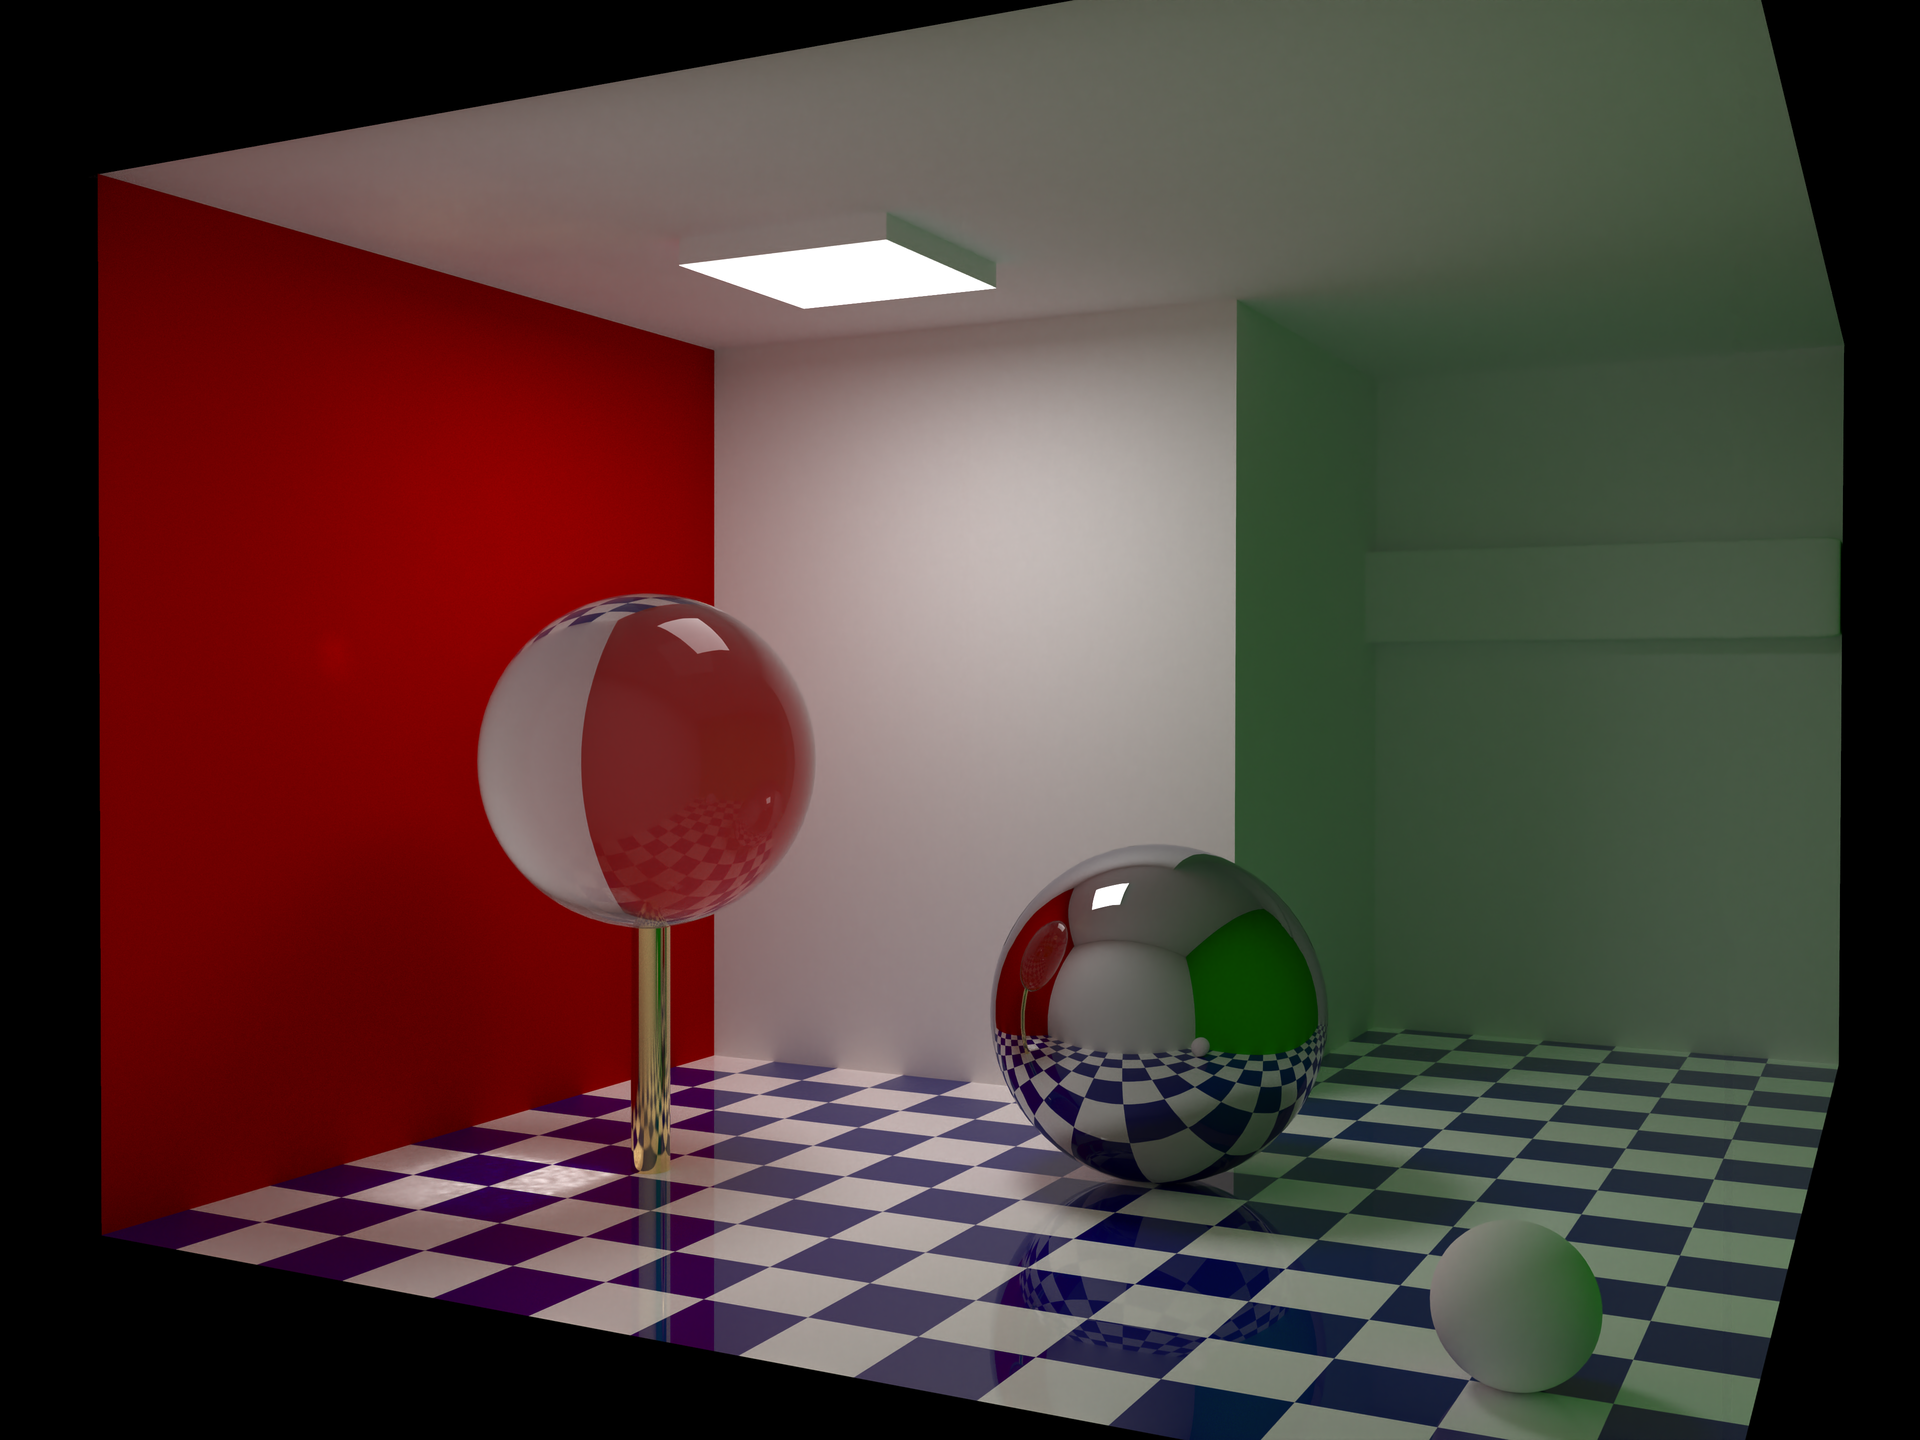
\includegraphics[width=0.75\textwidth]{global_illumination.png}
    \caption{Een plaatje gerenderd met \emph{global illumination}.}
    \label{fig:global_illumination}
\end{figure}

Eén van die technieken valt binnen de categorie van Monte-Carlosimulaties. Monte-Carlosimulaties gebruiken een willekeurig element  om in principe deterministische problemen op te lossen. Bij de rendervergelijking manifesteert dit zich in \emph{path tracing}. Bij \emph{path tracing} worden bij elk geraakt punt willekeurige nieuwe stralen afgevuurd, deze kaatsen door totdat ze een licht bereikt hebben. We komen hier bij hetzelfde probleem als eerder besproken terecht, de kans op het raken van een licht is niet erg groot. Hiertoe zijn twee belangrijke oplossingen. De eerste is \emph{bidirectional path tracing}, hier wordt tegelijk een straal vanuit de camera afgevuurd als van het licht. Na een bepaalde hoeveelheid kaatsen worden de twee verbonden waardoor er altijd een pad van de camera naar het licht is. De andere oplossing wordt \emph{importance sampling} genoemd. Daarbij is de distributie van de willekeurig afgekaatste lichtstralen niet uniform, er worden meer stralen richting de lichtbronnen afgekaatst. Hierdoor bereiken de stralen natuurlijk sneller de lichtbronnen. Met genoeg \emph{samples}\footnote{Hoeveelheid stralen} geeft dit algoritme een bijna perfecte benadering van de rendervergelijking, dat maakt het ook de industriële standaard van het moment. Maar het is relatief inefficiënt, dit komt doordat er met te weinig \emph{samples} veel ruis in het plaatje ontstaat. Dit is simpel te verklaren, omdat het algoritme fundamenteel willekeurig is zullen sommige pixels meer licht vinden dan die er direct naast. Puur omdat ze 'geluk' hadden. Slechts de limiet van het aantal \emph{samples} naar oneindig zou een werkelijk antwoord geven op de rendervergelijking. Daarom is er altijd een compromis met hoeveel tijd je wil besteden aan het renderen van een frame en de kwaliteit van het resultaat. Steeds vaker wordt kunstmatige intelligente gebruikt om die ruis weg te nemen of te verminderen \cite{MonteCarloDenoiser} maar in de industrie is dat nog steeds niet de norm. 

Een andere manier om integralen op te lossen is de eindige-elementenmethode

\subsection{Wat zijn polygonen?}
Een polygoon is, in zijn elementairste vorm, een eindig aantal 1ijnstukken die met elkaar verbonden zijn in een polygonale lijn. Dit houdt in dat elk uiteinde van een lijnstuk het begin van een nieuwe betekent. Bovendien betekent dit dat de lijnstukken altijd één keten vormen. 

Bij computer graphics hebben we het altijd over simpele polygonen. Deze polygonen snijden zichzelf niet en hebben geen gaten. Die simpele polygonen hebben een handige eigenschap, ze zijn altijd op te delen in driehoeken. Die driehoeken liggen altijd op een vlak, waar makkelijk een lijn mee te snijden valt. Vervolgens zijn er andere strategieën waarme te bepalen valt of dat punt in de driehoek ligt. 

Driedimensionale vormen worden met moderne rendertechnieken vrijwel altijd beschreven met deze polygonen. De vorm wordt dan een \emph{mesh} genoemd.

\subsection{Hoe wordt een mesh opgeslagen?}
Er zijn twee hoofdtechnieken: \emph{vertex-vertex meshes} \cite{VVSystems} en \emph{face-vertex meshes}. De \emph{vertex-vertex meshes} of VV-meshes bevatten één lijst die alle punten beschrijft. Daarnaast staan alle verbindingen die dat punt heeft met andere punten. In theorie minimaliseer je met deze techniek de geheugenbezetting. Echter maakt het het ontleden van driehoeken uit de vorm erg complex. Daarvoor zijn FV-meshes geschikter. Daar wordt van twee lijsten gebruik gemaakt. De eerste bevat weer alle punten, echter worden in plaats van de andere punten waarmee die verbonden zijn de verbonden vlakken beschreven. De andere lijst beschrijft al die vlakken en de hoekpunten ervan. De vlakken kunnen alleen driehoeken beschrijven, maar het eerder genoemde polygonale triangulatie principe betekent dat enige polygonale vorm hiermee beschreven kan worden.

\begin{figure}[h]
    \centering
    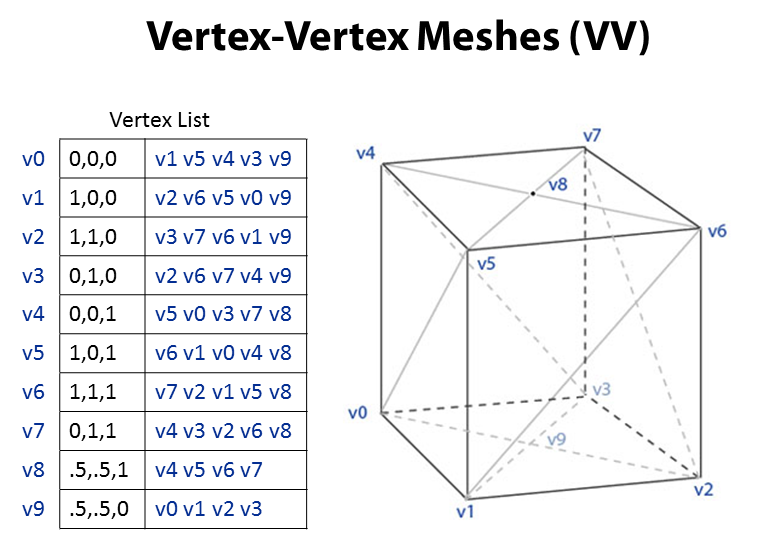
\includegraphics[width=0.75\textwidth]{Vertex-Vertex_Meshes.png}
    \caption{Voorbeeld van VV-representatie van een mesh.}
    \label{fig:vertex_vertex}
\end{figure}

\begin{figure}[h]
    \centering
    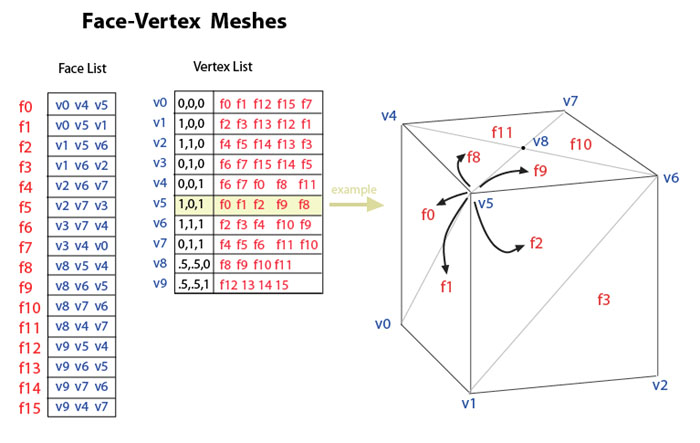
\includegraphics[width=0.75\textwidth]{Face-Vertex_Meshes.jpg}
    \caption{Voorbeeld van FV-representatie van een mesh.}
    \label{fig:face_vertex}
\end{figure}

\subsection{Wat is raymarching?}
Raymarching is een methode om het snijpunt van een straal en een vorm te vinden door iteratief stappen te zetten richting die vorm. De meest gebruikelijke methode hiervoor heet sphere tracing. Hierbij wordt gebruik gemaakt van de afstand van het originele punt tot het dichstbijzijnde van de vorm. In de richting van de straal wordt verplaatst met de afstand \(r\) tot dat dichtstbijzijnde punt. Dit wordt de locatie van het nieuwe punt. Op dat punt wordt het proces weer herhaald totdat de afstand onder een van te voren bepaalde grenswaarde valt.
\begin{algorithm}
\caption{Raymarch Algoritme}\label{euclid}
\begin{algorithmic}[1]
\Procedure{MarchRay}{pos, rot, obj, $\epsilon$}
\State $\textit{r} \gets \text{distance between }\textit{pos}\text{ and }\textit{obj}$
\While{$r  < \epsilon$}
\State $\textit{pos} \gets \textit{pos} + \textit{rot} \cdot r$
\State $\textit{r} \gets \text{distance between }\textit{pos}\text{ and }\textit{obj}$
\EndWhile
\Return $\textit{pos}$
\EndProcedure
\end{algorithmic}
\end{algorithm}

\subsection{Wat zijn SDFs?}
Het bepalen van de afstand van een punt tot het dichstbijzijnde punt op een vorm wordt gedaan met zogeheten \emph{signed distance}-functies. \emph{Signed} staat in deze term voor het feit dat aan de binnenkant van de vorm de functie een negatief getal geeft. De functie van een bol met middelpunt \(C\) en straal \(r\) is bijvoorbeeld als volgt:
\[\phi (x)=\left |x-C \right | -r\]
SDFs zijn enorm nuttig omdat we bewerkingen op deze formule toe kunnen passen waardoor we met vrijwel geen rekenkracht complexe vormen kunnen creëren. 

Neem vorm $\phi_1$ en vorm $\phi_2$. Als je de \emph{union}\footnote{De vormen samengevoegd} wil nemen van de vormen gebruik je de volgende simpelweg de volgende formule: 
\[\phi_{u(1,2)}=min(\phi_1, \phi_2)\]
De \emph{subtraction}\footnote{De ene vorm van de andere afgetrokken} wordt als volgt berekend:
\[\phi_{s(1,2)}=max(-\phi_1, \phi_2)\]
En de \emph{intersection}\footnote{Het deel wat bij beide vormen hoort} zo:
\[\phi_{i(1,2)}=max(\phi_1, \phi_2)\]
Dit worden de boolean operaties genoemd, en staan respectievelijk voor: OR, NOT en AND.

Een andere interessante operatie is de modulus, hiermee is het mogelijk om een vorm voor eeuwig te laten herhalen. Voor een periode $c$ en een SDF $\phi$ is de formule hiervoor:
\[\phi_{mod}= \phi +\frac{1}{2}c\mod{c}\]

\clearpage
\section{Hypothese}
\clearpage
\section{Ontwikkeling}
\subsection{Hardware}
\subsection{Software}
\subsubsection{Besturingssysteem}
Het uitvoeren en programmeren van de code zal volledig met Linux gedaan worden. Deze keuze is om meerdere redenen gemaakt. Ten eerste is Linux de standaardkeuze voor developers om te ontwikkelen. Windows en MacOS zijn ontwikkeld als product voor de gebruiker, terwijl Linux ontwikkeld is voor stabiliteit en betrouwbaarheid. Dit heeft als effect dat er met Linux veel minder tegen het besturingssysteem in gewerkt hoeft te worden. Bovendien zijn alle tools die gebruikt worden voor dit onderzoek FOSS\footnote{\textbf{F}ree and \textbf{O}pen \textbf{S}ource \textbf{S}oftware}, en daardoor voor zowel Windows als Linux beschikbaar. Dus qua support maakt het geen verschil.

Als distributie\footnote{Linux zelf is slechts een \emph{kernel} die de interactie tussen de hardware en de software regelt. Bovenop deze \emph{kernel} bestaan distributies die het een werkend besturingssysteem maken.} is voor Manjaro\footnote{https://manjaro.org/} gekozen. Dit is een fork van Arch Linux. Arch Linux staat erom bekend dat het altijd de nieuwste versie van software support. Dit komt doordat het een \emph{rolling release model} heeft, in tegenstelling tot \emph{fixed release}, waar distributies zoals Debian gebruik van maken. Bovendien heeft Arch Linux toegang tot de Arch User Repository (AUR). Dat is een enorme collectie van software die gebruikers zelf kunnen uploaden naar de Arch servers, met helpers zoals \emph{yay} kan je met één commando vrijwel alle software die beschikbaar is op GNU/Linux op de computer installeren. De combinatie van deze voordelen maken Arch Linux een erg aantrekkelijke distributie om te gebruiken als programmeur. Manjaro voegt de rest van de functies toe aan het besturingssysteem, zoals een Desktop Environment (DE) en een terminal.
\subsubsection{Programmeertaal}
Er zijn talloze programmmeertalen die geschikt zijn voor graphics programming. Daarom was de keuze voor de programmeertaal niet makkelijk. Zelf heb ik al jarenlang ervaring met Python\footnote{https://www.python.org/}, maar deze taal staat niet bekend om de snelheid. Dit komt doordat het een \emph{interpreted} taal is. Dat betekent dat de code live gelezen wordt wanneer gerund. Dit staat tegenover \emph{compiled} talen, die de code eerst compileren naar machinetaal. Die machinetaal is veel efficiënter te lezen door computers, waardoor de snelheid toeneemt. Een andere optie was Javascript, het grote voordeel van deze taal is dat hij speciaal voor het web gemaakt is. Hierdoor zou het delen van het gemaakte project met anderen zo simpel zijn als het doorsturen van een url. Bovendien maakt Javascript op moderne browsers gebruik van Just In Time (JIT) compilation. Dat is een combinatie tussen \emph{interpreted} en \emph{compiled} waar de code live omgezet wordt in machinetaal voordat het gerund wordt. Maar toch is zelfs Javascript niet snel genoeg. Bovendien missen beide talen iets wat erg belangrijk is in computer graphics: controle over het geheugen. Scènes kunnen enorm complex zijn dus het is belangrijk dat die zo efficiënt mogelijk in het geheugen geplaatst worden, en het geheugen moet weer gewist worden wanneer het niet meer gebruikt wordt. Python en Javascript geven allebei niet die controle, in plaats daarvan probeert de \emph{interpreter} zelf zo efficiënt mogelijk het geheugen te gebruiken. Om deze redenen heb ik gekozen voor C++, deze taal is in 1985 uitgevonden door Brane Stroustrup en wordt vandaag de dag nog door 20,17\% van Stack Overflow gebruikers gebruikt\cite{StackOverflowSurvey}. De taal is ontwikkeld als extensie voor C, waardoor het moderne functies heeft zoals \emph{Object Oriented Programming} (OOP) en datastructuren. Maar het heeft tegelijkertijd alle voordelen die C heeft als low-level taal. 
\subsubsection{Framework}
C++ heeft uit zichzelf nog geen grafische capabiliteiten. Daar is een framework voor nodig. Moderne grafische kaarten zijn allemaal gemaakt met speciale specificaties, die ervoor zorgen dat het besturingssysteem weet hoe hij moet communiceren met de GPU. Er zijn verschillende van deze specificaties met verschillende doelen. Zo heb je DirectX, die specifiek gemaakt is voor Windows. En wat algemenere API\footnote{\textbf{A}pplication \textbf{P}rogramming \textbf{I}nterface} is OpenGL (Open Graphics Library). Met C++ is het dan ook mogelijk om direct gebruik te maken van deze API, net als in de meeste programmeertalen. 

Maar toch heb ik daar niet voor gekozen. Dit is omdat OpenGL heel goed is in het implementeren van bestaande rendermethodes, waar de GPU ook voor ontwikkeld is. Dit maakt het ideaal voor het bouwen van videogames, omdat het daar heel snel in is. Maar minder voor dit specifieke onderzoek. Ik wil objectief vergelijken hoe de verschillende rendermethoden tegen elkaar opwegen, als de gebruikelijkere methodes heel goed geoptimaliseerd zijn door de GPU en OpenGL zou dat oneerlijk zijn en de data onbetrouwbaar maken. Daarom heb ik gekozen voor raylib\footnote{https://www.raylib.com/}. Raylib is een zeer minimalistische \emph{library} die alle basistools geven die we nodig hebben om te kunnen tekenen op een canvas, terwijl het tegelijkertijd razendsnel blijft. 
\subsubsection{Integrated Development Environment}
Ik ga al mijn programmeren doen in Visual Studio Code\footnote{https://code.visualstudio.com/} omdat het een mooie simpele text editor is die precies doet wat ik wil. Het geeft goede IntelliSense\footnote{Verzamelnaam voor tools die helpen in het schrijven van code zoals: code completion en informatie over parameters}, syntax highlighting en het geeft een goed overzicht van het project. Bovendien heeft het een enorme markt van plugins die het product nog meer verbeteren. Zo gebruik ik de Vim keybinds plugin om de efficiënte workflow van de editor Vim\footnote{https://www.vim.org/} te emuleren. 
\subsection{Programmeren}
\subsubsection{Specificaties}
Voor het onderzoek ga ik twee verschillende renderers ontwikkelen. De eerste gebruikt raytracing, en de objecten worden beschreven met raymarching. De tweede gebruikt ook raytracing alleen worden de objecten polygonaal beschreven. Het is voor het onderzoek belangrijk dat de twee algoritmes zo veel mogelijk op elkaar lijken, zodat het vergelijkende onderzoek iets objectiefs kan zeggen over de effectiviteit van de verschillende technieken. Vandaar dat hier eerst de specificaties worden beschreven waar de algoritmes aan zullen moeten doen. Deze specificaties kunnen uitgebreid worden of ingekort gebaseerd op de progressie over de tijd.

De renderer moet kunnen renderen vanuit een \textbf{camera} die een bepaalde positie heeft binnen de driedimensionale ruimte. De camera heeft ook een \emph{field of view} (fov), die aangeeft hoe breed het zichtveld is. Uit de camera komt uit elke pixel een \emph{ray} die snijdt met de \emph{viewport}. De resolutie van het beeldscherm wordt in het programma aangegeven. Waarschijnlijk willen we renderen op een resolutie van \(500\times 500\). De \emph{rays} worden beschreven als parametrische vergelijking. Hierdoor kan de parameter \(t\) gebruikt worden om de straal te snijden met de objecten. De objecten zijn uiteraard anders beschreven in de twee verschillende programma's, maar ze hebben wel delen gemeen. Zo heeft een object altijd een positie, een draaiing en een grootte. Verder wordt het materiaal van elk object beschreven met een kleur, de \emph{specularity} en het reflectievermogen. De kleur wordt beschreven met RGBA, met waarden op \([0, 255]\). De \emph{specularity} geeft de macht waarmee de cosinus die de verspreiding van de \emph{highlights} beschrijft wordt verheven. Het reflectievermogen is een getal op \([0, 1]\) die het aandeel van de kleur beschrijft die komt uit reflecties. Bovendien willen we een aantal primitieve vormen hebben die standaard beschikbaar zijn. Voor raymarching zal dit triviaal zijn aangezien elke vorm slechts een \emph{signed distance function} is. Maar voor het polygonale renderen moeten hier nog aparte algoritmes voor komen. De vormen die ondersteund moeten worden zijn als volgt:
\begin{itemize}
	\item Bol
	\item Vlak
	\item Driehoek
	\item Balk
	\item Ellipsoïde
	\item Cylinder
\end{itemize}

Verder zijn er ook verschillende soorten lichten mogelijk. Die nemen drie typen aan:
\begin{itemize}
	\item Ambient
	\item Point
	\item Directional
\end{itemize}
Alle lichten hebben een intensiteit, die aangeeft hoe vel dat licht is. Ambient lichten belichten de hele scène met een standaard hoeveelheid, er wordt hierbij dus geen rekening gehouden met schaduwen. Ambient lichten hebben maar één waarde: de intensiteit, die een waarde op \([0, 1]\) aanneemt. Point lichten hebben daarbij ook nog een positie, bovendien kan de intensiteit hoger dan 1 zijn. Directional lichten hebben geen positie maar een richting, en hebben ook een intensiteit die hoger kan zijn dan 1.

De camera, alle objecten en de lichten worden allemaal beschreven met een Scene() object. Die heeft de methodes AddSDFObject(), AddPolygon(), AddPolygonalPrimitive() en AddLight(). De scène zal in een los bestand van de rest van de code beschreven worden.
\subsubsection{Raylib uitproberen}
\subsubsection{Computer Graphics From Scratch}
Voor het bouwen van de raytracer is gebruik gemaakt van het boek \emph{Computer Graphics From Scratch} \cite{ComputerGraphicsFromScratch} van Gabriel Gambetta. Het boek beschrijft stap voor stap hoe men een renderer kan bouwen, de eerste helft gaat over een raytracer en de tweede helft een rasterizer. Het geeft een duidelijke beschrijving van de wiskundige theorie achter raytracen en stelt met pseudocode een structuur voor waarmee het geprogrammeerd kan worden. Aan het einde heb je een programma die kan raytracen met diffuse belichting, specular highlighting, schaduwen en reflecties. Het boek beschrijft alleen maar hoe bollen getekend kunnen worden, dus de hele implementatie van de raymarching zal zelf bedacht moeten worden. Daarbovenop is er ook geen implementatie van polygonen. 
\subsubsection{Raytracing}
De stralen worden aangegeven met een paramatervergelijking in de vorm:
\[P=O+t(V-O)\]
Hier is $P$ enig punt in de straal van $O$ naar $V$. $t$ geeft aan hoe ver op de straal punt $P$ is.

$(V-O)$ is gelijk aan de richting van de straal, dus die noemen we $\overrightarrow{D}$. Dan krijg je:
\[P=O+t\overrightarrow{D}\]

In het begin zal de raytracer alleen bollen kunnen tekenen, de vergelijking van punt $P$ op een bol met middenpunt $C$ en straal $r$ is:
\[|P-C|=r\]

De lengte van een vector is gelijk aan de wortel van het inwendig product met zichzelf. Het inwendig product wordt aangegeven als $\langle\overrightarrow{V},\overrightarrow{V} \rangle$. Dat geeft:
\[\langle P-C,P-C\rangle=r^2\]
Dit combineren met de vergelijking van de straal $P=O+t\overrightarrow{D}$ geeft:
\[\langle O+t\overrightarrow{D}-C,O+t\overrightarrow{D}-C\rangle=r^2\]
$O-C$ kunnen we opschrijven als $\overrightarrow{CO}$:
\[\langle{CO}+t\overrightarrow{D},\overrightarrow{CO}+t\overrightarrow{D}\rangle=r^2\]
Inwendige producten zijn bilineair, dit betekent dat:
\[\langle x+y,z\rangle=\langle x,z\rangle+\langle y,z\rangle\]
En:
\[\langle x,y+z\rangle=\langle x,y\rangle+\langle x,z\rangle\]
En:
\[\langle x,\lambda y\rangle=\lambda\langle x,y\rangle=\langle\lambda x,y\rangle\]
Hieruit kunnen we de vergelijking afsplitsen tot:
\[\langle \overrightarrow{CO},\overrightarrow{CO} \rangle + \langle t\overrightarrow{D},\overrightarrow{CO} \rangle + \langle \overrightarrow{CO},t\overrightarrow{D} \rangle + \langle t\overrightarrow{D},t\overrightarrow{D} \rangle = r^2\]

Verder zijn kruisproducten commutatief dus $\langle x,y\rangle=\langle y,x\rangle$.

Hieruit volgt:
\[\langle t\overrightarrow{D},t\overrightarrow{D} \rangle + 2\langle t\overrightarrow{D},\overrightarrow{CO} \rangle + \langle \overrightarrow{CO},\overrightarrow{CO} \rangle = r^2\]

Met de derde bilineairiteitsregel kunnen we dit weer omschrijven naar:
\[t^2\langle \overrightarrow{D},\overrightarrow{D} \rangle + t\left(2\langle \overrightarrow{D},\overrightarrow{CO} \rangle
\right) + \langle \overrightarrow{CO},\overrightarrow{CO} \rangle - r^2 = 0\]

Nu heeft het de vorm aangenomen van de kwadratische vergelijking, die we op kunnen lossen met de ABC-formule.
\[\{t_1, t_2\}=\frac{-b\pm \sqrt{b^2-4ac}}{2a}\]
Hierbij geldt dus:
\[a=\langle \overrightarrow{D},\overrightarrow{D}\rangle\]
\[b=2\langle \overrightarrow{CO},\overrightarrow{D}\rangle\]
\[c=\langle \overrightarrow{CO},\overrightarrow{CO}\rangle-r^2\]

In de code wordt dit als volgt geschreven:
\begin{lstlisting}[language=C++]
Vector2 IntersectRaySphere(Vector3 O, Vector3 D, Sphere sphere) {
    double r = sphere.radius;
    Vector3 CO = subtract(O, sphere.center);

    double a = dot(D, D);
    double b = 2 * dot(CO, D);
    double c = dot(CO, CO) - r*r;

    double discriminant = b*b-4*a*c;

    if (discriminant < 0) {
        return (Vector2){1E9, 1E9};
    }

    double t1 = (-b + sqrt(discriminant))/(2*a);
    double t2 = (-b - sqrt(discriminant))/(2*a);

    return (Vector2){t1, t2};
}
\end{lstlisting}

Voor de situatie zonder oplossing wordt $\{10^9,10^9\}$ teruggegeven. Later wordt gecheckt of de teruggeven waarde boven een bepaalde grens ligt, waarna hij wordt weggeworpen.

\begin{lstlisting}[language=C++]
for (int x = -canvas.width/2; x < canvas.width/2; x++) {
    for (int y = -canvas.height/2; y < canvas.height/2; y++) {
        Vector3 D = vp.CanvasToViewport(canvas, x, y);
        Color color = TraceRay(O, D, 1, 1E9, scene, 3);
        canvas.PutPixel(x, y, color);
    }
}
\end{lstlisting}

Hiervoor wordt gebruik gemaakt van de viewport, die als volgt is gedefiniëerd:
\begin{lstlisting}[language=C++]
class Viewport {
    public:
        double width;
        double height;

        double projection_plane_distance;

        Viewport(double w, double h, double ppd);
        Viewport();

        Vector3 CanvasToViewport(Canvas canvas, int x, int y);
};
\end{lstlisting}

De viewport is een virtueel vlak die op een bepaalde afstand $d$ van de camera staat. De stralen worden afgevuurd door deze viewport. Uit een punt $P$ op de viewport kan de vector $\overrightarrow{OP}$ gehaald worden. Dit is hetzelfde als de $\overrightarrow{D}$ uit de parametervergelijking van de straal.

De volgende functie converteert screenspace coördinaten naar de coördinaten op de viewport.
\begin{lstlisting}[language=C++]
Vector3 Viewport::CanvasToViewport(Canvas canvas, int x, int y) {
    return (Vector3){x*width/canvas.width, y*height/canvas.height, projection_plane_distance};
}
\end{lstlisting}

\begin{figure}[h]
    \centering
    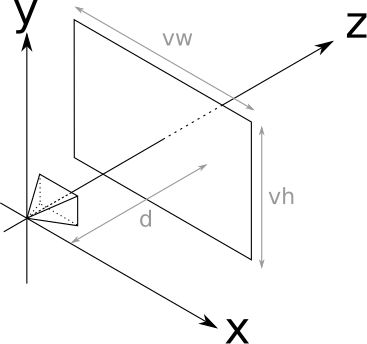
\includegraphics[width=0.75\textwidth]{viewport.png}
    \caption{Projectie van camera op viewport.}
    \label{fig:viewport}
\end{figure}

Het afvuren van de stralen vanuit de viewport wordt gedaan met de TraceRay() functie.

\begin{lstlisting}[language=C++]
Color TraceRay(Vector3 O, Vector3 D, double t_min, double t_max, Scene scene) {   
    std::pair<Sphere, double> closest_intersection = ClosestIntersection(O, D, t_min, t_max, scene);
    Sphere closest_sphere = closest_intersection.first;

    if (closest_t==1E9) {
        return RAYWHITE;
    }

    return closest_sphere.material.color;
}
\end{lstlisting}
De functie geeft een kleur terug, in dit vroegste geval is dat gewoon de kleur van het object. Die kleur wordt vervolgens voor de bijbehorende pixel getekend.

Er wordt gebruik gemaakt van de ClosestIntersection() functie. 

\begin{lstlisting}[language=C++]
std::pair<Sphere, double> ClosestIntersection(Vector3 O, Vector3 D, double t_min, double t_max, Scene scene) {
    double closest_t = 1E9;
    Sphere closest_sphere;

    for (Sphere sphere: scene.spheres) {
        Vector2 t_points = IntersectRaySphere(O, D, sphere);
        double t1 = t_points.x;
        double t2 = t_points.y;

        if ((t1 > t_min && t1 < t_max)&&(t1<closest_t)) {
            closest_t = t1;
            closest_sphere = sphere;
        }

        if ((t2 > t_min && t2 < t_max)&&(t2<closest_t)) {
            closest_t = t2;
            closest_sphere = sphere;
        }
    }

    return std::make_pair(closest_sphere, closest_t);
}
\end{lstlisting}
Deze geeft terug welke bol het dichst bij is, en hoe ver die bol precies is. 

Samen geeft dit de eerste versie van de raytracer. We initialiseren de scène als volgt:

\begin{lstlisting}[language=C++]
Viewport vp(1, 1, 1);

Scene scene(vp);

scene.AddSphere(Sphere(
    (Vector3){0, -1, 3},
    1,
    ObjectMaterial (
        (Color){255, 0, 0, 255},
        500,
        0.2
    )
));

scene.AddSphere(Sphere(
    (Vector3){2, 0, 4},
    1,
    ObjectMaterial (
        (Color){0, 0, 255, 255},
        500,
        0.2
    )
));

scene.AddSphere(Sphere(
    (Vector3){-2, 0, 4},
    1,
    ObjectMaterial (
        (Color){0, 255, 0, 255},
        500,
        0.2
    )
));

scene.AddSphere(Sphere(
    (Vector3){0, -5001, 0},
    5000,
    ObjectMaterial (
        (Color){255, 255, 0, 255},
        500,
        0
    )
));
\end{lstlisting}

In het begin wordt een Scene() object aangemaakt. Daaraan kunnen vervolgens objecten aan toegevoegd worden. Dat Scene() object ziet er zo uit:

\begin{lstlisting}[language=C++]
class Scene {
    public:
        Viewport vp;

        std::vector<Sphere> spheres;

        Scene(Viewport viewport);

        void AddSphere(Sphere sphere);
};
\end{lstlisting}

Alle bollen worden in een vector opgeslagen. Die bollen zijn zelf weer een aparte klasse, die als volgt is gedefiniëerd:

\begin{lstlisting}[language=C++]
class Sphere {
    public:
        Vector3 center;
        double radius;

        ObjectMaterial material;

        Sphere(Vector3 center, double radius, ObjectMaterial material);
        Sphere();
};
\end{lstlisting}

Ieder object heeft een ObjectMaterial, in deze eerste versie beschrijft die alleen de kleur:

\begin{lstlisting}[language=C++]
class ObjectMaterial {
    public: 
        Color color;

        ObjectMaterial(Color color);
        ObjectMaterial();
};
\end{lstlisting}

Hierna wordt de eerder beschreven loop over elke pixel gerund, hierdoor krijgen we onze eerste render.
\begin{figure}[h]
    \centering
    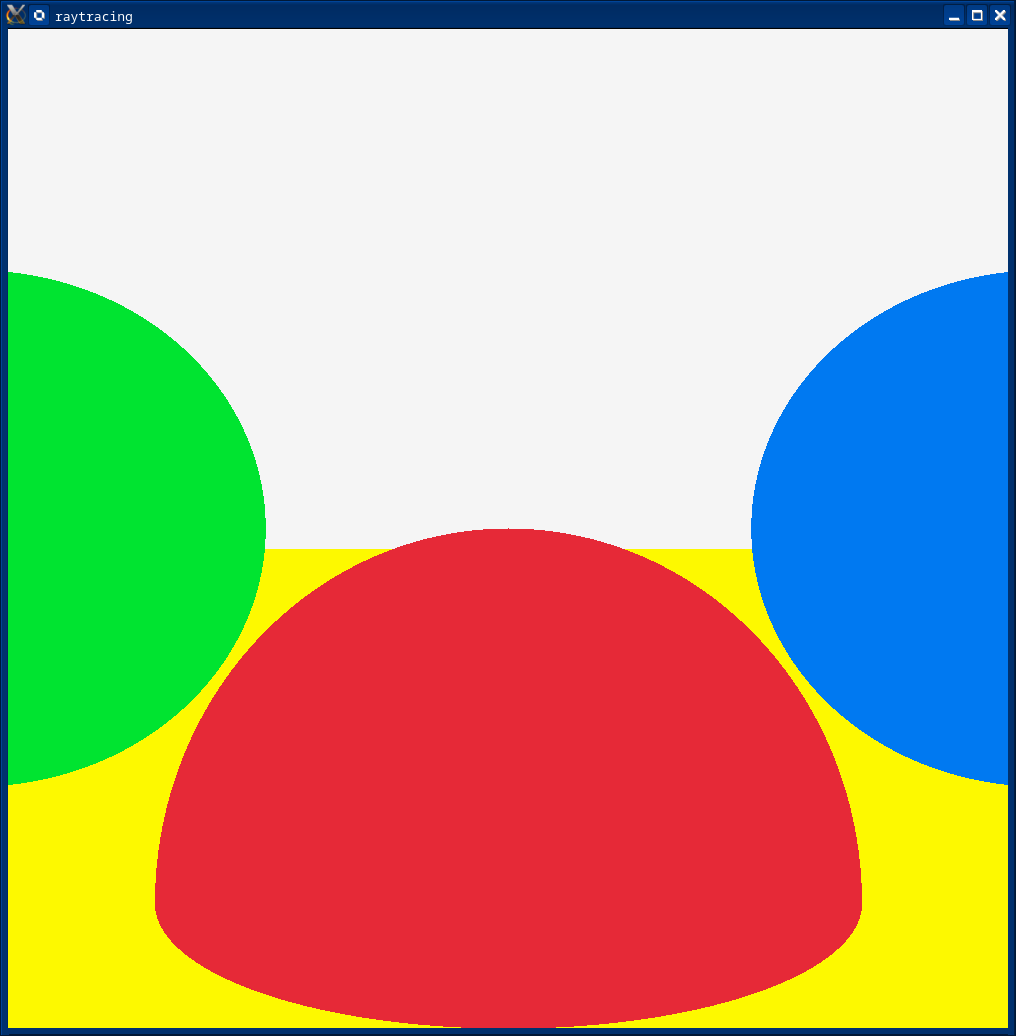
\includegraphics[width=0.50\textwidth]{renders/first_raytraced.png}
    \caption{De eerste render gemaakt met de raytracer.}
    \label{fig:first_raytraced}
\end{figure}

\subsubsection{Diffusion}
Diffusie in het Phong-Model. 

\begin{figure}[h]
    \centering
    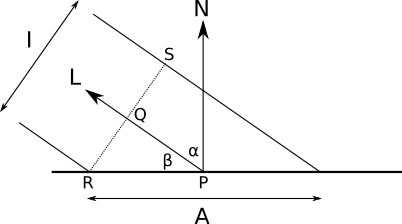
\includegraphics[width=0.50\textwidth]{diffuse-diagram.png}
    \caption{Diagram die laat zien hoe licht op een oppervlakte terecht komt.}
    \label{fig:diffuse-diagram}
\end{figure}


In figuur \ref{fig:diffuse-diagram} raakt lichtstraal $\overrightarrow{L}$ het object in P met hoek $\alpha$ tot normaal $\overrightarrow{N}$. De lichtstraal heeft intensiteit $I$, en is verspreidt over oppervlakte $A$. Dit betekent dat de intensiteit per eenheid oppervlakte $\frac{I}{A}$ is. In een rechte driehoek geldt: 
\[\cos{\alpha}=\frac{A}{S}\]

Hier is $A$ de aanliggende zijde en $S$ de schuine zijde. In het bovenstaande diagram is dat gelijk aan $\frac{I}{A}$.

Ook geldt dat:
\[\cos \alpha = \frac{\langle \overrightarrow{N},\overrightarrow{L}\rangle}{|\overrightarrow{N}||\overrightarrow{L}|}\]

Dus: 

\[\frac{I}{A} = \frac{\langle \overrightarrow{N},\overrightarrow{L}\rangle}{|\overrightarrow{N}||\overrightarrow{L}|}\]

Hieruit kunnen we de volgende algemene formule voor diffusie opstellen, met een som voor elke lichtbron met intensiteit $I_i$ en richting $\overrightarrow{L_i}$. Verder is $I_A$ de ambient belichting.

\[I_P=I_A+\sum_{i=l}^{n}I_i\frac{\langle \overrightarrow{N}, \overrightarrow{L_i} \rangle}{|\overrightarrow{N}||\overrightarrow{L_i}|}\]

De normaal van de bol met middelpunt $C$ in punt $P$ wordt zo bepaald:
\[\overrightarrow{N}=\frac{P-C}{|P-C|}\]

Door te delen met $|P-C|$ wordt de vector genormaliseerd, waardoor de lengte 1 wordt.

De volgende functie wordt gebruikt voor het berekenen van het licht:

\begin{lstlisting}[language=C++]
double ComputeLighting(Vector3 P, Vector3 N, Vector3 V,  Scene scene) {
    double i = 0.0;
    Vector3 L;

    for (Light light: scene.lights) {
        if (light.type == 0) {
            i += light.intensity;
        } else {
            if (light.type == 1) {
                L = subtract(light.position, P);
            } else if (light.type == 2) {
                L = light.direction;
            }

            // Diffuse
            double n_dot_l = dot(N, L);
            if (n_dot_l > 0) {
                i += light.intensity * n_dot_l/magnitude(L);
            }
        }
    }
    return i;
}
\end{lstlisting}

$P$ is het punt op de vorm, $N$ de normaal en $L$ de richting van het licht. Aan het Scene() object is nu ook een vector van de lichten in de scène toegevoegd. Die lichten zijn gedefiniëerd als volgt:

\begin{lstlisting}[language=C++]
class Light {
    public:
        int type; // 0: ambient; 1: point; 2: directional
        double intensity;

        Vector3 position;
        Vector3 direction;

        Light();
        Light(int t, double i);
        Light(int t, double i, Vector3 pos_or_rot);
};
\end{lstlisting}

De functie heeft het argument $t$, wat voor type staat. Er zijn drie types: ambient, directional en point. Die staan voor 1, 2 en 3 respectievelijk. Het initialiseren van een ambient licht gaat met de volgende functie:

\begin{lstlisting}[language=C++]
Light::Light(int t, double i) {
    type = t;
    intensity = i;
    position = (Vector3){0, 0, 0};
    direction = (Vector3){0, 0, 0};
}
\end{lstlisting}

En voor rotationele en positionele lichten gaat het zo:

\begin{lstlisting}[language=C++]
Light::Light(int t, double i, Vector3 pos_or_rot) {
    type = t;
    intensity = i;
    if (type == 1) {
        position = pos_or_rot;
        direction = (Vector3){0, 0, 0};
    } else if (type == 2) {
        position = (Vector3){0, 0, 0};
        direction = pos_or_rot;
    }
}
\end{lstlisting}

We voegen aan de scène de volgende lichten toe:

\begin{lstlisting}[language=C++]
scene.AddLight(Light(
    0, // Ambient
    0.2
));

scene.AddLight(Light(
    1, // Point
    0.6,
    (Vector3){2, 1, 0}
));

scene.AddLight(Light(
    2, // Directional
    0.2,
    (Vector3){1, 4, 4}
));
\end{lstlisting}

In de TraceRay() functie vermenigvuldigen we nu de originele kleur met de teruggegeven intensiteit. 

\begin{lstlisting}[language=C++]
Color TraceRay(Vector3 O, Vector3 D, double t_min, double t_max, Scene scene) {   
    std::pair<Sphere, double> closest_intersection = ClosestIntersection(O, D, t_min, t_max, scene);
    Sphere closest_sphere = closest_intersection.first;
    double closest_t = closest_intersection.second;

    if (closest_t==1E9) {
        return RAYWHITE;
    }

    Vector3 P = add(O, multiply(D, closest_t));
    Vector3 N = subtract(P, closest_sphere.center);
    N = multiply(N, 1/magnitude(N));
    return multiply(closest_sphere.material.color, ComputeLighting(P, N, multiply(D, -1), scene));

}
\end{lstlisting}

\begin{figure}[h]
    \centering
    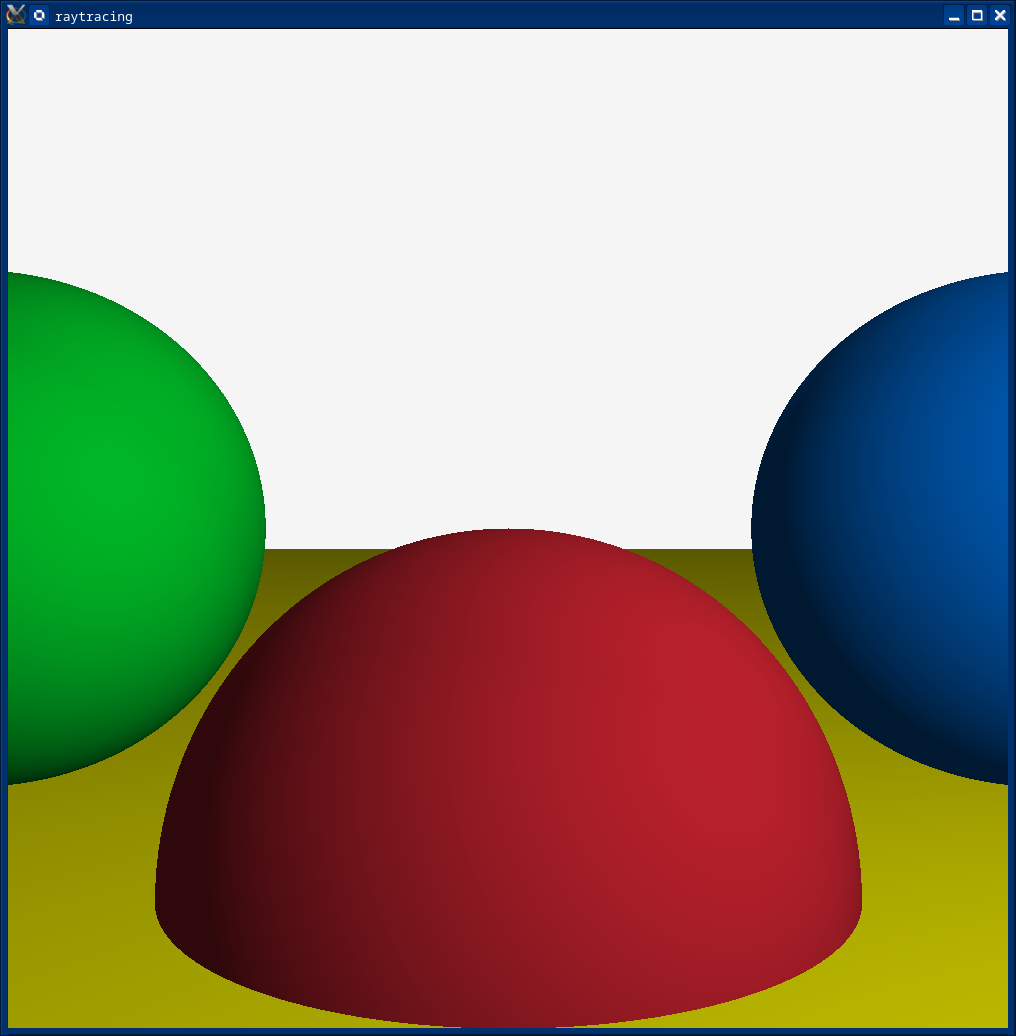
\includegraphics[width=0.50\textwidth]{renders/diffused.png}
    \caption{De renderer, nu met diffuse oppervlakten.}
    \label{fig:diffused}
\end{figure}

\subsubsection{Specular Highlights}

Voor speculaire reflectie wordt het licht niet in alle richtingen weerkaatst, maar meer in de richting tegenover de vector van inkomend licht gespiegeld in de normaal. De distributie van het teruggekaatste licht kunnen we met een cosinus functie aangeven. Die geeft een duidelijk distributie rondom de y-as. We verheffen de cosinus tot een bepaalde macht $s$, om te bepalen hoe scherp de reflecties zijn.

\begin{figure}[h]
    \centering
	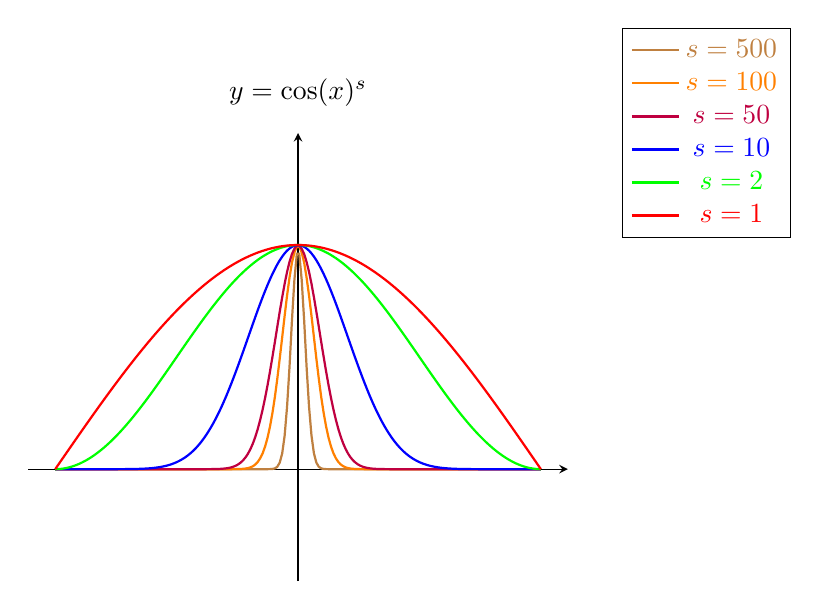
\begin{tikzpicture}
	\begin{axis}[
		xtick=\empty,
		ytick=\empty,
		xmin=-100,
		xmax=100,
		ymin=-0.5,
		ymax=1.5,
		axis x line=center,
		axis y line=center,
		legend style={at={(1.1,1)},anchor=west, title={$y = \cos(x)^s$}},
	]
	\addlegendentry[brown]{$s=500$};
	\addlegendentry[orange]{$s=100$};
	\addlegendentry[purple]{$s=50$};
	\addlegendentry[blue]{$s=10$};
	\addlegendentry[green]{$s=2$};
	\addlegendentry[red]{$s=1$};
	\addplot[color=brown, thick, samples=200, domain=-90:90] {cos(x)^500};
	\addplot[color=orange, thick, samples=200, domain=-90:90] {cos(x)^100};
	\addplot[color=purple, thick, samples=200, domain=-90:90] {cos(x)^50};
	\addplot[color=blue, thick, samples=200, domain=-90:90] {cos(x)^10};
	\addplot[color=green, thick, samples=200, domain=-90:90] {cos(x)^2};
	\addplot[color=red, thick, samples=200, domain=-90:90] {cos(x)^1};
	\end{axis}
	\end{tikzpicture}
    \caption{Cosinus functies verheven tot verschillende machten $s$.}
    \label{fig:cosini}
\end{figure}

We kunnen $\ora{L}$ ontleden in $\ora{L_P}$ en $\ora{L_N}$, waar $\ora{L_N}$ evenwijdig is aan $\ora{N}$ en $\ora{L_N}$ loodrecht staat op $\ora{N}$.

\begin{figure}[h]
    \centering
    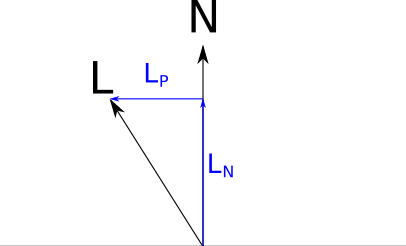
\includegraphics[width=0.50\textwidth]{L_decomposition.png}
    \caption{$\protect\overrightarrow{L}$ ontleden in componenten $\protect\overrightarrow{L_P}$ en $\protect\overrightarrow{L_N}$}
    \label{fig:L_decomposition}
\end{figure}

Omdat $\left|\ora{N}\right| = 1$, geldt $\left|\ora{L_N}\right|=\langle\ora{N},\ora{L}\rangle$. $\ora{L_N}$ is evenwijdig met $\ora{N}$ dus $\ora{L_N}=\ora{N}\langle\ora{N},\ora{L}\rangle$.

$\ora{L}=\ora{L_P}+\ora{L_N}$ dus $\ora{L_P}=\ora{L}-\ora{L_N}=\ora{L}-\ora{N}\langle\ora{N},\ora{L}\rangle$.

\begin{figure}[h]
    \centering
    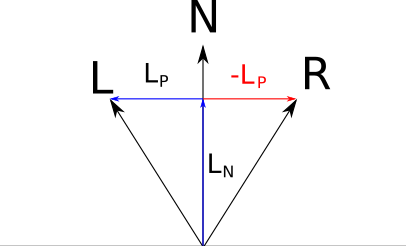
\includegraphics[width=0.50\textwidth]{LR_Calculation.png}
    \caption{Het berekenen van $\protect\ora{L_R}$}
    \label{fig:LR_Calculation}
\end{figure}

$\ora{R}$ is aan de andere kant van $\ora{N}$ en heeft dezelfde hoogte als $\ora{R}$ dus $\ora{R}=\ora{L_N}-\ora{L_P}$

Als we hierin de eerder verkregen formules substitueren krijgen we:

\[\ora{R}=\ora{N}\langle\ora{N},\ora{L}\rangle-\ora{L}+\ora{N}\langle\ora{N},\ora{L}\rangle\]
\[\ora{R}=2\ora{N}\langle\ora{N},\ora{L}\rangle-\ora{L}\]

Verder weten we dat:
\[\cos\left(\angle\left(\ora{R}, \ora{V}\right)\right)=\frac{\langle\ora{R},\ora{V}\rangle}{\left|\ora{R}\right|\left|\ora{V}\right|}\]

Hieruit volgt de volgende formule voor speculaire reflecties:
\[I_S=I_L\left(\frac{\langle\ora{R},\ora{V}\rangle}{\left|\ora{R}\right|\left|\ora{V}\right|}\right)^s\]

Dit kunnen we samenvoegen met de eerder vergaarde formule voor diffusie voor een volledige belichtingsformule:

\[
I_P=
I_A+
\sum_{i=l}^{n}I_i\cdot\left[
\frac{\langle \overrightarrow{N}, \overrightarrow{L_i} \rangle}{|\overrightarrow{N}||\overrightarrow{L_i}|}+
\left(\frac{\langle\ora{R_i},\ora{V}\rangle}{\left|\ora{R_i}\right|\left|\ora{V}\right|}\right)^s\right]
\]

In de code ziet de ComputeLighting() functie er nu als volgt uit:

\begin{lstlisting}[language=C++]
double ComputeLighting(Vector3 P, Vector3 N, Vector3 V, double s, Scene scene) {
    double i = 0.0;
    Vector3 L;

    for (Light light: scene.lights) {
        if (light.type == 0) {
            i += light.intensity;
        } else {
            if (light.type == 1) {
                L = subtract(light.position, P);
            } else if (light.type == 2) {
                L = light.direction;
            }

            // Diffuse
            double n_dot_l = dot(N, L);
            if (n_dot_l > 0) {
                i += light.intensity * n_dot_l/magnitude(L);
            }

            // Specular
            if (s != -1) {
                Vector3 R = subtract(multiply(N, 2* dot(N, L)), L);
                double r_dot_v = dot(R, V);
                if (r_dot_v > 0) {
                    i += light.intensity * pow(r_dot_v/(magnitude(R)*magnitude(V)), s);
                }
            }
        }
    }
    return i;
}
\end{lstlisting}

We stellen dat een object geen speculaire reflecties heeft als $s=-1$. 

We voegen aan de ObjectMaterial() klasse de specular eigenschap toe:

\begin{lstlisting}[language=C++]
class ObjectMaterial {
    public: 
        Color color;
        double specular;

        ObjectMaterial(Color color, double specular);
        ObjectMaterial();
};
\end{lstlisting}

Nu kunnen we de bollen renderen met speculaire reflecties.

\begin{figure}[h]
    \centering
    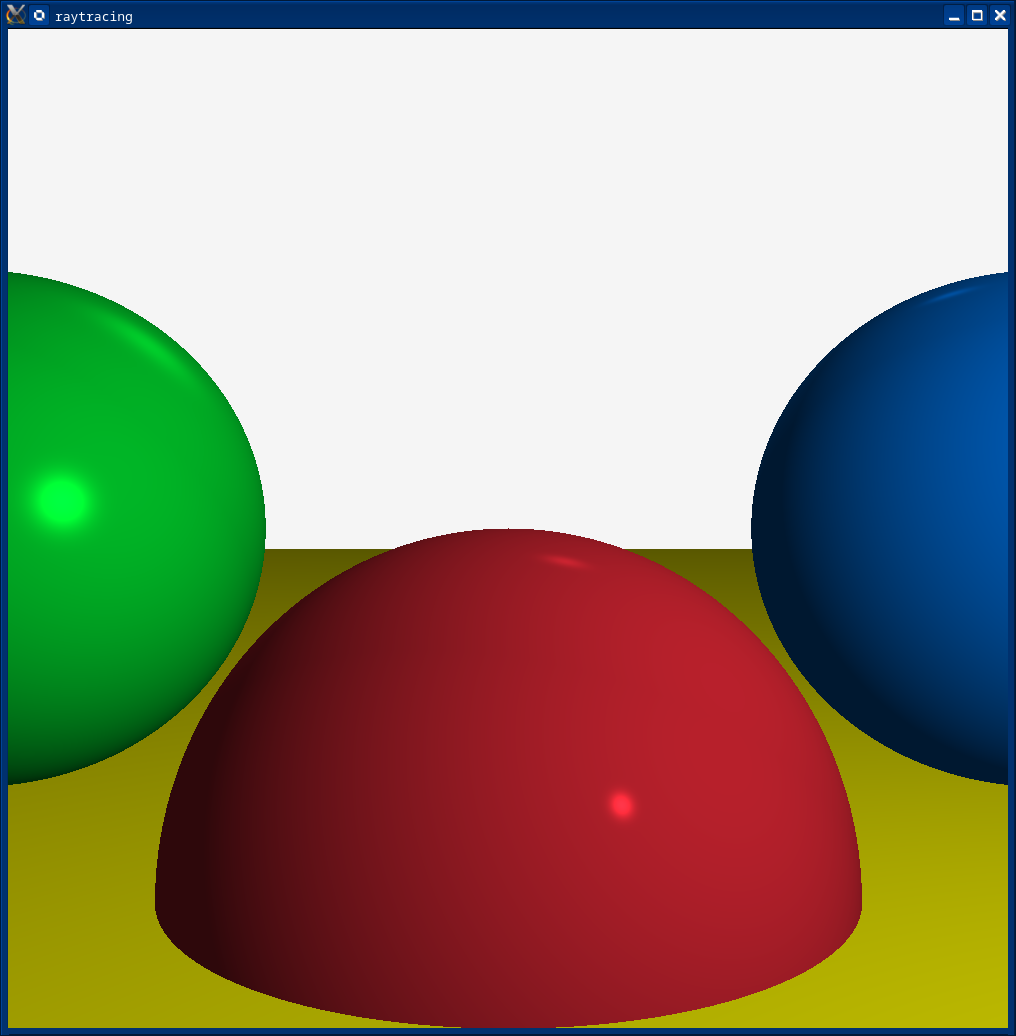
\includegraphics[width=0.50\textwidth]{renders/specular.png}
    \caption{De bollen gerenderd met speculaire reflecties. De rode bol heeft een hogere waarde $s$ dan de groene bol.}
    \label{fig:specular}
\end{figure}

\subsubsection{Schaduwen}
Om te weten waar schaduwen getekend moeten worden wordt een nieuwe straal vanaf een punt op de vorm afgevuurd richting de camera. Als er een andere vorm tussenzit berekenen we voor dat punt niet de diffuse en speculaire reflectie. We kunnen hiervoor de eerder geschreven ClosestIntersection() functie hergebruiken. De ComputeLighting functie ziet er dan als volgt uit:

\begin{lstlisting}[language=C++]
double ComputeLighting(Vector3 P, Vector3 N, Vector3 V, double s, Scene scene) {
    double i = 0.0;
    Vector3 L;

    for (Light light: scene.lights) {
        if (light.type == 0) {
            i += light.intensity;
        } else {
            if (light.type == 1) {
                L = subtract(light.position, P);
            } else if (light.type == 2) {
                L = light.direction;
            }

            // Shadow Check
            double shadow_t = ClosestIntersection(P, L, 0.001, 1E9, scene).second;
            if (shadow_t != 1E9) {
                continue;
            } 

            // Diffuse
            double n_dot_l = dot(N, L);
            if (n_dot_l > 0) {
                i += light.intensity * n_dot_l/magnitude(L);
            }

            // Specular
            if (s != -1) {
                Vector3 R = subtract(multiply(N, 2* dot(N, L)), L);
                double r_dot_v = dot(R, V);
                if (r_dot_v > 0) {
                    i += light.intensity * pow(r_dot_v/(magnitude(R)*magnitude(V)), s);
                }
            }
        }
    }
    return i;
}
\end{lstlisting}

Dit zijn alle aanpassingen die gemaakt moeten worden aan de code.

\begin{figure}[h]
    \centering
    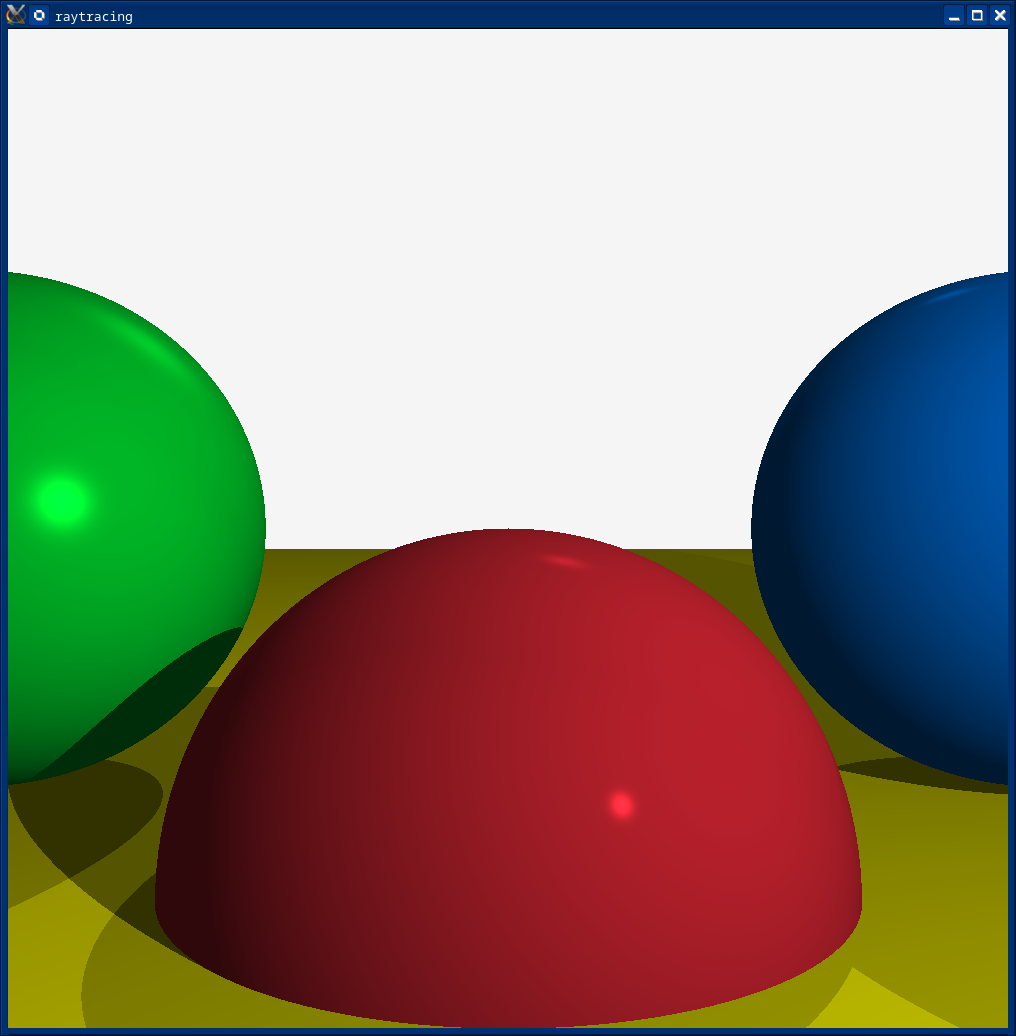
\includegraphics[width=0.50\textwidth]{renders/schaduw.png}
    \caption{De bollen gerenderd met schaduwen.}
    \label{fig:schaduw}
\end{figure}

\subsubsection{Reflecties}

Om reflecties te tekenen moet de TraceRay() functie vanaf het raakpunt opnieuw uitgevoerd worden in de tegenovergestelde richting van de normaal. De formule voor reflectie was eerder vastgesteld als:
\[\ora{L}=2\ora{N}\langle\ora{N},\ora{R}\rangle-\ora{R}\]

Daaruit is de volgende functie geschreven:

\begin{lstlisting}[language=C++]
Vector3 ReflectRay(Vector3 R, Vector3 N) {
    return subtract(multiply(N, 2 * dot(N, R)), R);
}
\end{lstlisting}

We passen de TraceRay() functie recursief toe:
\begin{lstlisting}[language=C++]
Color TraceRay(Vector3 O, Vector3 D, double t_min, double t_max, Scene scene, int recursion_depth) {   
    std::pair<Sphere, double> closest_intersection = ClosestIntersection(O, D, t_min, t_max, scene);
    Sphere closest_sphere = closest_intersection.first;
    double closest_t = closest_intersection.second;

    if (closest_t==1E9) {
        return RAYWHITE;
    }

    Vector3 P = add(O, multiply(D, closest_t));
    Vector3 N = subtract(P, closest_sphere.center);
    N = multiply(N, 1/magnitude(N));
    Color local_color = multiply(closest_sphere.material.color, ComputeLighting(P, N, multiply(D, -1), closest_sphere.material.specular, scene));

    double r = closest_sphere.material.reflective;
    if (recursion_depth <=0 || r <= 0) {
        return local_color;
    }

    Vector3 R = ReflectRay(multiply(D, -1), N);
    Color reflected_color = TraceRay(P, R, 0.001, 1E9, scene, recursion_depth - 1);

    return add(multiply(local_color, 1 - r), multiply(reflected_color, r)); 

}
\end{lstlisting}

Aan de ObjectMaterial() klasse is de laatste nieuwe eigenschap reflective toegevoegd, de reflectie wordt met deze waarde vermenigvuldigd:

\begin{lstlisting}[language=C++]
class ObjectMaterial {
    public: 
        Color color;
        double specular;
        double reflective;

        ObjectMaterial(Color color, double specular, double reflective);
        ObjectMaterial();
};
\end{lstlisting}

Als reflective lager is dan 0 stellen we dat er geen reflecties zijn voor dat object. Deze kleine toevoegingen maken de basis van de raytracer af.

\begin{figure}[h]
    \centering
    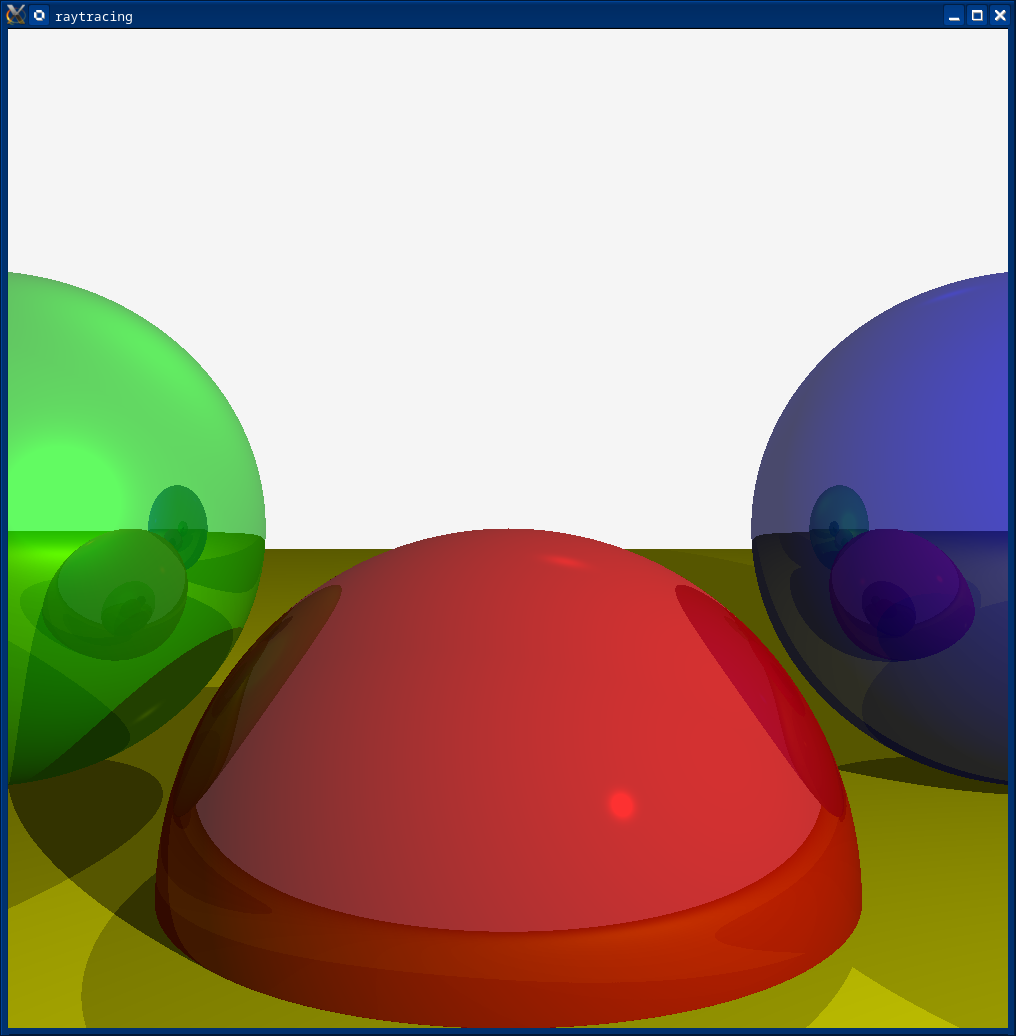
\includegraphics[width=0.50\textwidth]{renders/reflection.png}
    \caption{De bollen gerenderd met reflecties.}
    \label{fig:reflection}
\end{figure}

\subsubsection{Raymarching}

De IntersectRaySphere() functie wordt vervangen door MarchRay(). Verder is het Sphere() object nu weg. In plaats daarvan spreken we over een SDFObject(), die een methode SDF() heeft.

\begin{lstlisting}[language=C++]
double marchRay(Vector3 O, Vector3 D, SDFObject *object, double max_distance, int max_marching_steps, double max_depth) {
    double depth = magnitude(D);

    for (int i = 0; i < max_marching_steps; i++) {
        double distance = object->SDF(add(O, multiply(D, depth)));
        if (distance < max_distance) {
            return depth;
        }

        depth += distance;


        if (depth >= max_depth) {
            return 1E9;
        }
    }

    return 1E9;
}
\end{lstlisting}

Er wordt steeds een stap in de richting van de straal gezet met de grootte van de afstand tot het object, totdat de afstand lager is dan een bepaalde aangegeven grenswaarde.

Verder moet de normaal nog berekend worden. De normaal is gelijk aan de gradiënt van het oppervlakte:

\[\ora{N} = \text{normalize}(\nabla f(p))\]

Waar $f(p)$ de SDF is.

De definitie van de gradiënt zegt:

\[\nabla f(p)=\left\{\frac{df(p)}{dx},\frac{df(p)}{dy},\frac{df(p)}{dz}\right\}\]

De afgeleide is te benaderen met:

\[\frac{df(p)}{dx}\approx\frac{f\left(p+\begin{pmatrix} \epsilon \\ 0 \\ 0 \end{pmatrix}\right)-f\left(p-\begin{pmatrix} \epsilon \\ 0 \\ 0 \end{pmatrix}\right)}{2\epsilon}\]

Hieruit volgt:

\[
\ora{N}=\text{normalize}\begin{pmatrix} 
f\left(p+\begin{pmatrix} \epsilon \\ 0 \\ 0 \end{pmatrix}\right)-f\left(p-\begin{pmatrix} \epsilon \\ 0 \\ 0 \end{pmatrix}\right) \\
f\left(p+\begin{pmatrix} 0 \\ \epsilon \\ 0 \end{pmatrix}\right)-f\left(p-\begin{pmatrix} 0 \\ \epsilon \\ 0 \end{pmatrix}\right) \\
f\left(p+\begin{pmatrix} 0 \\ 0 \\ \epsilon \end{pmatrix}\right)-f\left(p-\begin{pmatrix} 0 \\ 0 \\ \epsilon \end{pmatrix}\right)
\end{pmatrix}\]

\subsubsection{SDFs}
\subsubsection{SDF operaties}
\subsubsection{Transformaties}
\subsubsection{Driehoeken}
\subsubsection{Mesh Representatie}
\subsubsection{Polygonale primitieven}
\subsubsection{Radiosity}z
\subsubsection{Interface}
\subsubsection{Meten}
\clearpage
\section{Methode}
\subsection{Variabelen}
\subsection{Meetmethoden}
\clearpage
\section{Resultaten}
\subsection{Snelheid}
\subsection{Geheugenbezetting}
\subsection{Renders}
\clearpage
\section{Nauwkeurigheidsanalyse}
\clearpage
\section{Conclusie}
\clearpage
\section{Discussie}
\clearpage
\section{Nawoord}
Bedankt aan mijn moeder Arria Gosman.
Bedankt aan Ina, voor haar mentale steun.
\clearpage
\section{Literatuurlijst}
\bibliographystyle{apalike}
\bibliography{refs}
\clearpage
\section{Logboek}
\begin{adjustbox}{angle=270}
\begin{tabular}{ | c | c c c c c | }
\hline
Activiteit & Datum & Tijd (m) & Totale tijd (h) &       \% Voltooid \\
\hline
Programmeren & 20220906 & 45 & 0.8 & 0.94\% \\
Programmeren & 20220908 & 30 & 1.3 & 1.56\% \\
Gesprek met begeleider & 20220909 & 20 & 1.6 & 1.98\% \\
Programmeren & 20220921 & 90 & 3.1 & 3.85\% \\
Inhoudsopgave Opzet & 20220928 & 35 & 3.7 & 4.58\% \\
Schrijven Theorie/Achtergrond Renderen & 20220930 & 45 & 4.4 & 5.52\% \\
Opzetten \LaTeX \space Document & 20221002 & 120 & 6.4 & 8.02\% \\
\hline
\end{tabular}
\end{adjustbox}

\end{document}